\documentclass[10pt,twocolumn,letterpaper]{article}

\usepackage{fontspec}
%\usepackage[vietnamese]{babel}
\usepackage[margin=0.75in]{geometry}
\usepackage{amsmath,amssymb,amsfonts,amsthm}
\usepackage{graphicx}
\usepackage{booktabs}
\usepackage{hyperref}
\usepackage{xcolor}
\usepackage{algorithm}
\usepackage{algorithmic}
\usepackage{microtype}
\usepackage{cite}
\usepackage{subcaption}

\hypersetup{
    colorlinks=true,
    linkcolor=blue,
    citecolor=teal,
    urlcolor=magenta
}

\newtheorem{theorem}{Định lý}
\newtheorem{lemma}{Bổ đề}
\newtheorem{definition}{Định nghĩa}

\title{\textbf{Khử Lượng Tử Hóa Mạng Đồ Thị Lượng Tử Tương Biến Nông: Thiên Kiến Quy Nạp Tuần Hoàn trong Truyền Thông Điệp Phân Tử}}

\author{
    \textbf{Nguyễn Trọng Lưu}, \textbf{Phạm Minh Hiếu}, \textbf{Phan Quốc Anh}, \textbf{Đỗ Xuân Chợ}\thanks{Tác giả liên hệ: \texttt{chodx@ptit.edu.vn}} \\
    \textit{Học viện Công nghệ Bưu chính Viễn thông (PTIT), Hà Nội, Việt Nam}
}
\date{}

\begin{document}

\maketitle

\begin{abstract}
Các mạch lượng tử tham số hóa (PQC) đã cho thấy những kết quả đầy hứa hẹn trong việc dự đoán tính chất điện tử của phân tử, tuy nhiên nguồn gốc của lợi thế này so với các mô hình cơ sở cổ điển vẫn chưa thực sự rõ ràng. Chúng tôi chỉ ra rằng lợi thế này không bắt nguồn từ hiện tượng vướng víu đa qubit mà đến từ một cơ chế cổ điển: các phép quay đơn qubit vốn dĩ tính toán các chuỗi Fourier cắt cụt, cung cấp một hệ cơ sở tuần hoàn gọn nhẹ mà các hàm kích hoạt đơn điệu không thể biểu diễn hiệu quả ở mức ngân sách tham số thấp. Để khai thác hiểu biết sâu sắc này, chúng tôi giới thiệu \textbf{PRISM}, một mạng GNN truyền thông điệp tương biến $\mathrm{E}(3)$ thay thế các hàm kích hoạt tiêu chuẩn bằng các hàm kích hoạt nội tuần hoàn hình sin (SIREN). Ở cùng số lượng tham số ($2{,}527$), PRISM đạt kết quả tương đương hoặc vượt trội một PQC 4-qubit trên toàn bộ các mục tiêu điện tử của QM9 và vượt qua PaiNN trên bốn trong số sáu tính chất. Việc mở rộng độ sâu mạch lên $L = 16$ tầng và số lượng qubit lên $n_q = 8$ xác nhận rằng các mạch lượng tử tiệm cận nhưng không bao giờ vượt qua năng lực biểu diễn cổ điển của PRISM, trong khi phải chịu sự suy giảm tốc độ huấn luyện lên tới $540\times$. Hơn nữa, lợi thế tuần hoàn vẫn duy trì bền bỉ trên toàn bộ tập dữ liệu QM9 ($N = 110{,}000$, 5 hạt giống, $q_{\mathrm{FDR}} \le 0.055$) và \textit{mở rộng} một cách đơn điệu từ $35.7\%$ lên $51.3\%$ khi dung lượng mô hình vượt qua ngưỡng $100{,}000$ tham số. Kết quả của chúng tôi xác lập các hàm kích hoạt nội tuần hoàn như một thiên kiến quy nạp mạnh mẽ không cần phần cứng cho học sâu hình học phân tử.
\end{abstract}

\section{Giới thiệu}
\label{sec:intro}

Các mạch lượng tử tham số hóa (PQC) là những ứng viên hàng đầu trong kỷ nguyên ngắn hạn nhằm tìm kiếm lợi thế lượng tử thực tiễn trong học máy~\cite{Kandala:2017vok, Cerezo:2020mtn}. Dự đoán tính chất phân tử là một miền ứng dụng tự nhiên: các phân tử tồn tại trong không gian Euclid 3 chiều với các đối xứng $\mathrm{E}(3)$ liên tục mà PQC có thể tuân thủ một cách tự nhiên, và các quy luật vật lý nền tảng vốn mang bản chất cơ học lượng tử~\cite{satorras2022enequivariantgraphneural, thomasTensorFieldNetworks2018}. Thật vậy, khi được tích hợp vào các mạng nơ-ron đồ thị tương biến, các PQC nông luôn vượt trội hơn các mô hình đường cơ sở cổ điển có cùng số tham số trên các mục tiêu orbital điện tử như HOMO, LUMO, và khe HOMO-LUMO trong chế độ dữ liệu ít (Hình~\ref{fig:scaling_law}).

Nhưng \textit{tại sao} chúng lại hoạt động hiệu quả? Giả định phổ biến cho rằng sự vướng víu lượng tử hoặc khả năng biểu đạt trong không gian Hilbert đem lại ưu thế đó. Chúng tôi chỉ ra rằng giả định này là không chính xác. Thông qua các phân tích triệt tiêu (ablation) có hệ thống trên 20 hạt giống ngẫu nhiên, chúng tôi chứng minh rằng sự vướng víu đa qubit đóng góp không đáng kể vào hiệu năng của PQC trên các mục tiêu phân tử. Cơ chế thực sự hoàn toàn mang tính cổ điển: các phép quay đơn qubit $R_Y(x)$, $R_Z(x)$ vốn dĩ tính toán các chuỗi Fourier cắt cụt~\cite{Schuld:2020enb, Perez-Salinas:2019pjx}, cung cấp một hệ cơ sở tuần hoàn gọn nhẹ mà các hàm kích hoạt đơn điệu tiêu chuẩn ($\tanh$, SiLU) không thể biểu diễn một cách hiệu quả ở mức ngân sách tham số tương đương. Đây là một khoảng cách về dung lượng biểu diễn, chứ không phải một khoảng cách lượng tử.

Chẩn đoán này mang tính xây dựng: nếu ưu thế của PQC bắt nguồn từ tính tuần hoàn, chúng ta có thể tái tạo nó hoàn toàn bằng phương pháp cổ điển bằng cách đặt các hàm kích hoạt tuần hoàn \textit{bên trong} các tầng truyền thông điệp tương biến. Trong khi SIREN~\cite{sitzmann2020siren} giới thiệu hàm kích hoạt hình sin cho các biểu diễn nơ-ron ẩn trong thị giác máy tính, và các kiến trúc phân tử hiện có sử dụng hàm lượng giác cho mã hóa \textit{đầu vào} (hàm điều hòa cầu trong TFN~\cite{thomasTensorFieldNetworks2018}, NequIP~\cite{batznerE3equivariantGraphNeural2021}, MACE~\cite{batatiaMACEHigherOrder2022}), chưa có công trình nào trước đây đưa hàm kích hoạt tuần hoàn vào bên trong các \textit{tầng ẩn} của mạng đồ thị tương biến. Chúng tôi giới thiệu \textbf{PRISM}, một mạng GNN truyền thông điệp tương biến $\mathrm{E}(3)$ thay thế các hàm kích hoạt đơn điệu bằng $\sin(\omega_0 \mathbf{W} \mathbf{x} + \mathbf{b})$ trong các MLP xử lý cạnh. Ở cùng số lượng tham số, PRISM đạt kết quả tương đương hoặc vượt trội PQC trên toàn bộ các mục tiêu điện tử mà không cần đến phần cứng lượng tử.

\paragraph{Đóng góp nghiên cứu.}
\begin{itemize}
    \item Chúng tôi cô lập cơ chế mang lại lợi thế cho PQC trên các mục tiêu điện tử của phân tử: nó bắt nguồn từ năng lực biểu diễn lượng giác đơn qubit, chứ không phải sự vướng víu đa qubit (Mục~\ref{sec:mechanism}).
    \item Chúng tôi giới thiệu \textbf{PRISM}, mạng GNN truyền thông điệp tương biến đầu tiên sở hữu các hàm kích hoạt \textit{nội} tuần hoàn hình sin, đạt kết quả tương đương hoặc vượt trội PQC ở mức đồng tham số và vượt qua PaiNN trên bốn trong số sáu mục tiêu QM9 (Mục~\ref{sec:periodic_egnn}).
    \item Chúng tôi chứng minh tính đầy đủ cổ điển trên các chế độ mở rộng quy mô mạch: việc mở rộng độ sâu PQC lên $L = 16$ tầng và bề rộng qubit lên $n_q = 8$ xác nhận rằng sự vướng víu lượng tử sâu không mang lại thêm bất kỳ lợi thế biên nào so với biểu diễn cạnh tuần hoàn hai tầng của PRISM, trong khi việc thực thi cổ điển mang lại tốc độ huấn luyện nhanh hơn $540\times$ (Mục~\ref{sec:depth_qubit_scaling}).
    \item Chúng tôi chứng minh rằng lợi thế tuần hoàn duy trì bền bỉ ở toàn bộ quy mô ($N = 110{,}000$, 5 hạt giống, $q_{\mathrm{FDR}} \le 0.055$; $p = 0.0035$ trên HOMO, $p = 0.0424$ trên LUMO, $p = 0.0547$ trên Gap) và \textit{mở rộng một cách đơn điệu} từ $35.7\%$ lên $51.3\%$ khi dung lượng mô hình vượt qua ngưỡng tiên tiến lên tới $100{,}127$ tham số (Mục~\ref{sec:param_scaling}).
    \item Chúng tôi cung cấp một phương pháp luận thống kê chặt chẽ (triệt tiêu giai thừa, kiểm chứng phổ Fourier, và hiệu chỉnh Benjamini-Hochberg FDR trên 48 giả thuyết) có thể áp dụng cho các nghiên cứu đối chuẩn QML trong tương lai (Mục~\ref{sec:init_ablation}, Phụ lục~\ref{sec:appendix_fdr}, SM~D).
\end{itemize}

\begin{figure*}[t]
    \centering
    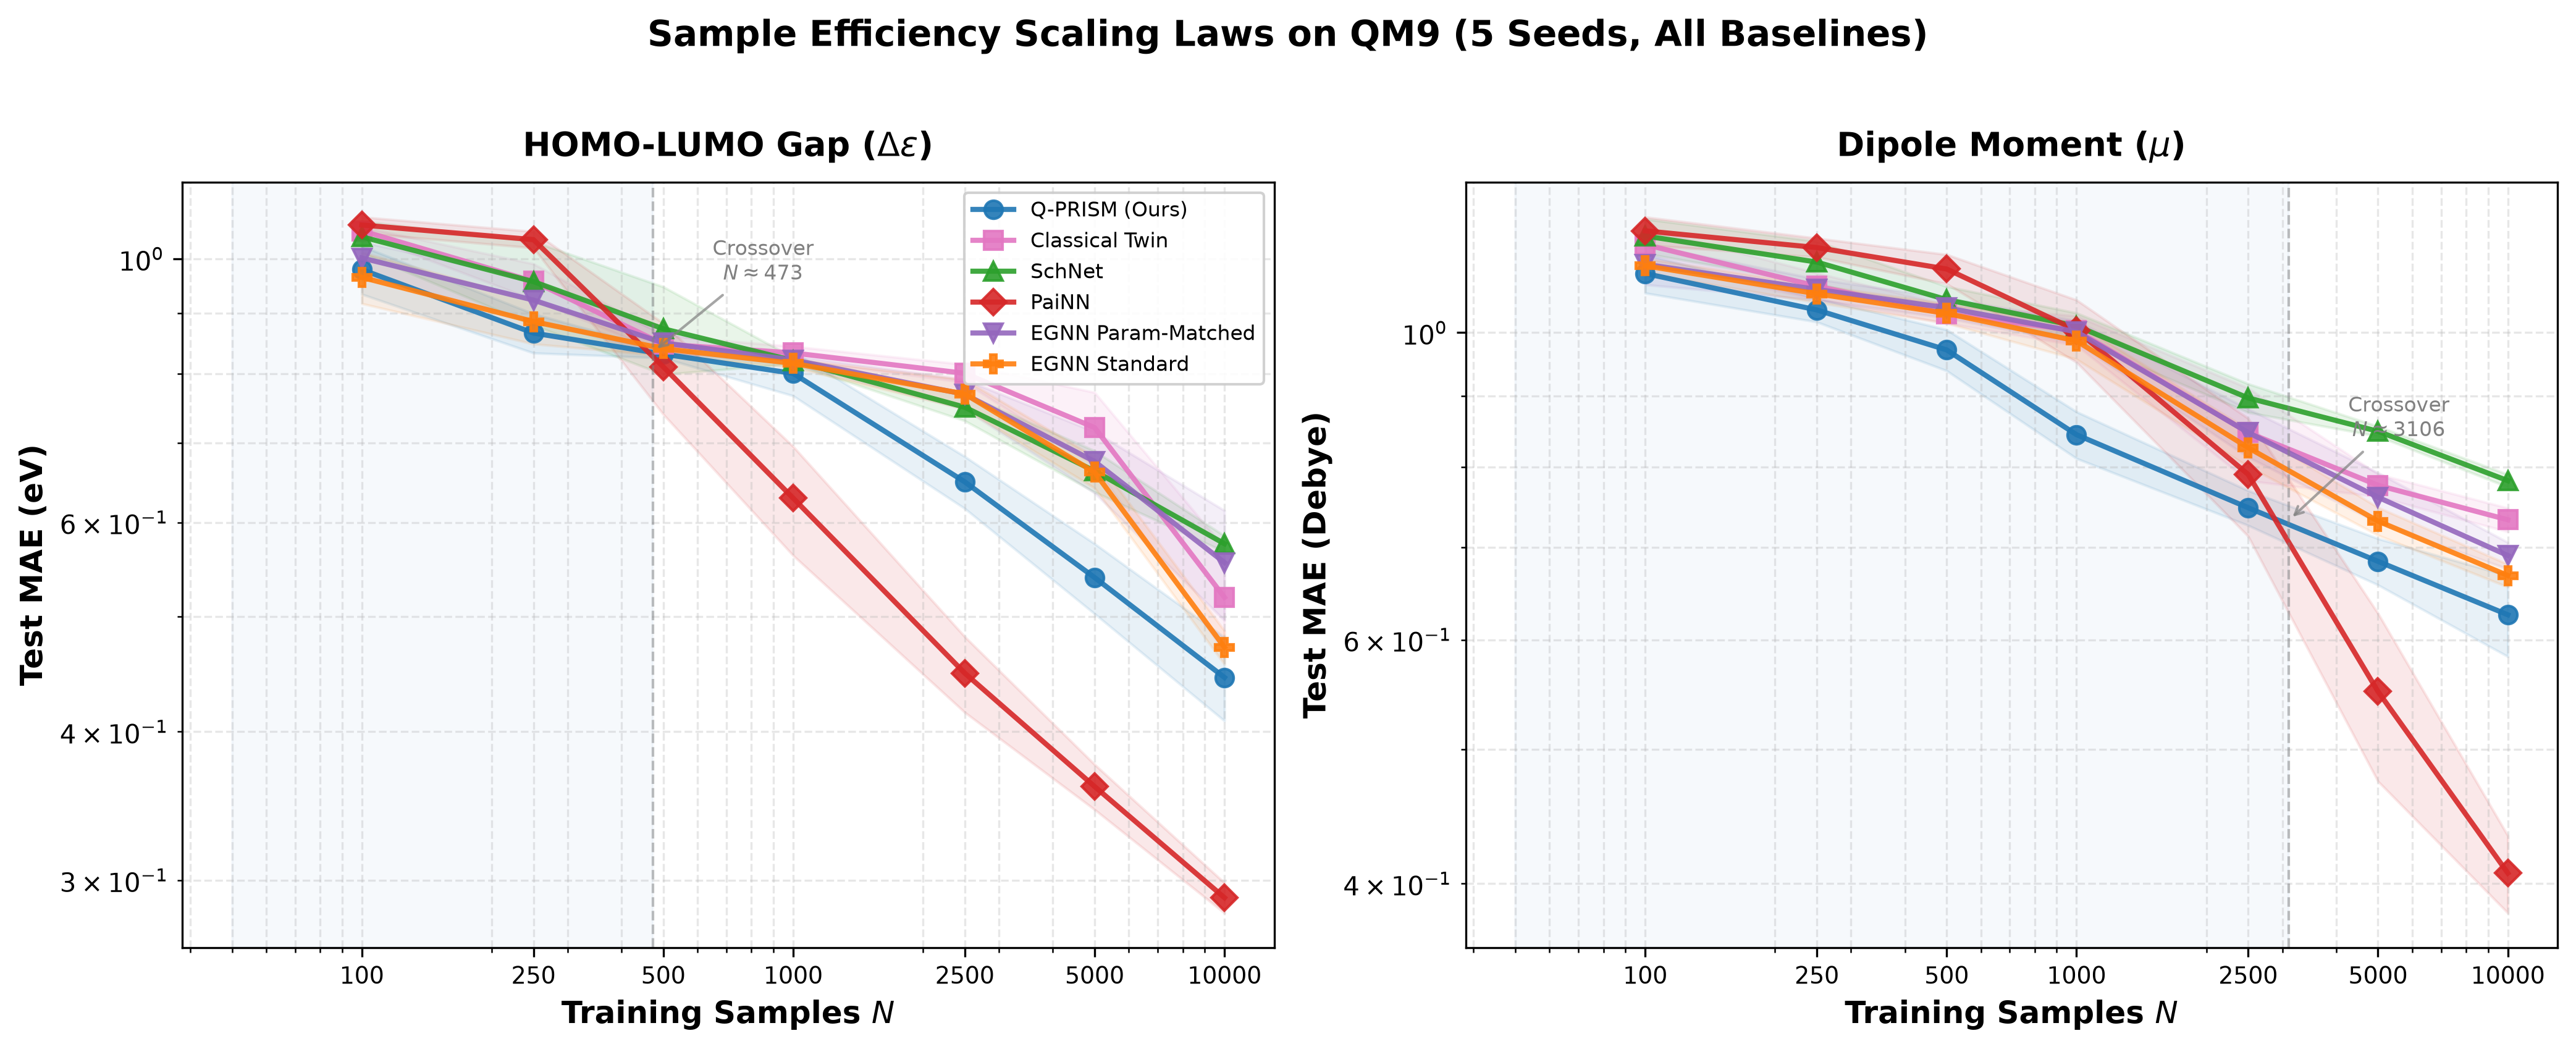
\includegraphics[width=0.88\textwidth]{figures/figure1_scaling_law.png}
    \caption{\textbf{Quy luật Mở rộng Hiệu quả Mẫu trên QM9 trên các Kích thước Mẫu $N \in [100, 10{,}000]$:} Các đường cong mở rộng log-log cho khe HOMO-LUMO $\Delta\epsilon$ (trái, eV) và Mômen Lưỡng cực $\mu$ (phải, Debye) trên 5 hạt giống ngẫu nhiên độc lập (trung bình $\pm$ độ lệch chuẩn). Q-PRISM ($2{,}527$\,tham số) được đối chuẩn với Bản song sinh Cổ điển ($\tanh$, $2{,}527$\,p), SchNet ($2{,}473$\,p), PaiNN ($2{,}721$\,p), EGNN Khớp Tham số ($2{,}497$\,p), và EGNN Tiêu chuẩn ($4{,}289$\,p). Trong chế độ khan hiếm dữ liệu ($N \le 500$), Q-PRISM vượt trội hơn tất cả các đường cơ sở. Khi kích thước mẫu tăng lên, biểu diễn vô hướng-vector kết hợp của PaiNN giao cắt với Q-PRISM tại $N \approx 473$ cho Gap và $N \approx 3{,}106$ cho Mômen Lưỡng cực, trong khi Q-PRISM luôn duy trì ưu thế trước các mô hình cơ sở tương biến vô hướng (EGNN, SchNet).}
    \label{fig:scaling_law}
\end{figure*}

\section{Công trình Liên quan}
\label{sec:related}

\paragraph{Học sâu Hình học Cổ điển.}
Các mạng GNN tương biến cho bài toán dự đoán tính chất phân tử đã đạt độ chính xác cao trên các tập dữ liệu hóa học lượng tử (xem bài tổng quan của No{\'e} et al.~\cite{Noe:2019yup}). Các kiến trúc tiêu biểu bao gồm các mô hình truyền thông điệp bất biến (EGNN~\cite{satorras2022enequivariantgraphneural}, SchNet~\cite{schütt2017schnetcontinuousfilterconvolutionalneural}, PhysNet~\cite{unkePhysNetNeuralNetwork2019}), các kiến trúc định hướng và góc (DimeNet++~\cite{klicperaFastUncertaintyAwareDirectional2020}, GemNet~\cite{klicperaGemNetUniversalDirectional2021}, PaiNN~\cite{schuttEquivariantMessagePassing2021}), các phương pháp tensor bậc cao (TFN~\cite{thomasTensorFieldNetworks2018}, NequIP~\cite{batznerE3equivariantGraphNeural2021}, MACE~\cite{batatiaMACEHigherOrder2022}, Equiformer~\cite{liao2023equiformer}), và các khung tương biến có khả năng mở rộng quy mô (TorchMD-Net~\cite{tholke2022torchmdnet}, Allegro~\cite{musaelianLearningLocalEquivariant2022}, LEFTNet~\cite{duNewPerspectiveBuilding2023}). Khung MPNN của Gilmer et al.~\cite{gilmer2017neural} thống nhất phần lớn các mô hình này dưới một hình thức truyền thông điệp chung. Tuy nhiên, tất cả đều chia sẻ một lựa chọn thiết kế chung: các hàm kích hoạt đơn điệu, tuyến tính cục bộ (SiLU, Swish, hoặc softplus dịch chuyển) bên trong các MLP truyền thông điệp và cập nhật nút. Chúng tôi thách thức lựa chọn mặc định này.

\paragraph{Thiên kiến Phổ và Hàm kích hoạt Tuần hoàn.}
Trong lý thuyết học sâu, Rahaman et al.~\cite{rahaman2019spectral} chứng minh rằng các mạng nơ-ron tiêu chuẩn thể hiện \textit{thiên kiến phổ}: gradient descent ưu tiên học các thành phần Fourier tần số thấp, với biên độ Fourier tần số cao suy giảm nhanh theo cấp $\mathcal{O}(\|k\|^{-(d+1)})$.
Tancik et al.~\cite{tancik2020fourier} phân tích điều này qua lý thuyết Nhân Tiếp tuyến Nơ-ron (NTK), chứng minh rằng các MLP tọa độ thất bại trong việc biểu diễn các cấu trúc không gian tinh vi trừ khi các đầu vào được ánh xạ sang các đặc trưng Fourier.
Sitzmann et al.~\cite{sitzmann2020siren} giới thiệu SIREN (Sinusoidal Representation Networks), chứng minh rằng các hàm kích hoạt tuần hoàn ($\sin(\omega_0 W x + b)$) kết hợp với lược đồ khởi tạo có cơ sở nguyên lý (phân phối đều được điều chỉnh theo $\omega_0$) có thể vượt qua hoàn toàn thiên kiến phổ và cho phép huấn luyện ổn định các đạo hàm ở mọi bậc.
Mặc dù SIREN là chuẩn mực cho biểu diễn nơ-ron ẩn trong thị giác máy tính~\cite{sitzmann2020siren}, các hàm kích hoạt \textit{nội} tuần hoàn chưa từng xuất hiện bên trong các MLP truyền thông điệp của mạng đồ thị tương biến. Các mô hình hình học hiện nay chỉ dùng hàm lượng giác cho \textit{mã hóa không gian đầu vào}, chẳng hạn như cơ sở xuyên tâm Bessel cầu trong DimeNet++~\cite{klicperaFastUncertaintyAwareDirectional2020} hoặc hàm điều hòa cầu trong NequIP~\cite{batznerE3equivariantGraphNeural2021} và MACE~\cite{batatiaMACEHigherOrder2022}, để lại toàn bộ các hàm kích hoạt tầng xuôi dòng ở dạng đơn điệu.

\paragraph{Khử lượng tử hóa và Các Giới hạn Căn bản của QML.}
Các nghiên cứu gần đây đặt dấu hỏi về việc liệu các lợi thế của PQC có thực sự phản ánh các tài nguyên lượng tử hay không. Huang et al.~\cite{Huang:2021qml} chỉ ra rằng sức mạnh mô hình QML phụ thuộc vào sự tương thích của thiên kiến quy nạp với dữ liệu chứ không phải bản thân phần cứng lượng tử; Schuld~\cite{Schuld:2021kernel} chứng minh rằng các mô hình lượng tử biến phân có giám sát tương đương một cách hình thức với các phương pháp nhân. Về mặt thực nghiệm, Schreiber et al.~\cite{Schreiber:2022roq} chứng minh rằng các PQC tính toán các chuỗi Fourier cắt cụt có thể bắt kịp bởi các mô hình đại diện cổ điển, K\"ubler et al.~\cite{kubler2021inductive} truy nguyên hiệu năng của nhân lượng tử về thiên kiến quy nạp hơn là phần cứng, và Pegg et al.~\cite{pegg2026isoqgnn} chỉ ra rằng các bản song sinh cổ điển đồng tham số có thể bắt kịp các mô hình lượng tử trong bài toán dự đoán khe HOMO-LUMO. Landman et al.~\cite{landman2023approximating} khẳng định rằng các PQC tải lại dữ liệu thực chất là các chuỗi Fourier cắt cụt đa chiều có thể xấp xỉ qua Đặc trưng Fourier Ngẫu nhiên với độ phức tạp mẫu đa thức. Điều này được củng cố vững chắc về mặt lý thuyết: Cerezo, Holmes et al.~\cite{Cerezo:2023nqf} xác lập \textit{tình thế lưỡng nan giữa khả năng huấn luyện và khả năng mô phỏng}, chứng minh rằng các PQC tránh được cao nguyên cằn cỗi (barren plateaus)~\cite{Cerezo:2020mtn, McClean:2018jps} thường nằm trong các lớp độ phức tạp có thể mô phỏng cổ điển, trong khi việc mở rộng sang các mạch sâu, vướng víu cao có nguy cơ gây ra hiện tượng tập trung độ đo hàm mũ~\cite{Thanasilp:2022agd}, buộc các nhân lượng tử suy biến về các hằng số tầm thường. Jerbi et al.~\cite{Jerbi:2021qnz} đã xác định các điều kiện cấu trúc khắt khe cần thiết để duy trì ưu thế trước các bộ học cổ điển. Theo khuôn khổ khử lượng tử hóa của Tang~\cite{Tang:2018lmw}, phương pháp của chúng tôi cô lập cơ chế chính xác đằng sau hiệu năng biểu kiến của PQC và tái tạo nó bằng mô hình cổ điển.

\paragraph{Học Máy Lượng tử Tương biến.}
Các khuôn khổ toán học hình thức đã tích hợp các ràng buộc đối xứng vào các mạch lượng tử tham số hóa.
Meyer et al.~\cite{meyer2023exploiting} phát triển một khuôn khổ nhóm đối xứng để xây dựng các PQC tương biến, chứng minh rằng việc áp đặt các đối xứng nhóm làm thu hẹp không gian giả thuyết hiệu dụng của mạch về các không gian con có ý nghĩa vật lý, cải thiện cả hiệu quả mẫu lẫn khả năng tổng quát hóa.
Skolik et al.~\cite{skolik2023equivariant} chỉ ra rằng các mạch lượng tử tương biến đạt khả năng tổng quát hóa tốt hơn trên các tác vụ học tập đối xứng với ít tham số huấn luyện hơn.
Tính tương biến $\mathrm{E}(3)$ của Q-PRISM đạt được ở \textit{cấp độ kiến trúc đồ thị} (thông qua các đầu vào cạnh bất biến và các cập nhật tọa độ tương biến) chứ không phải qua thiết kế mạch đối xứng, bổ trợ cho các hướng tiếp cận ở cấp độ mạch này. PRISM kế thừa cùng các bảo đảm tương biến ở cấp đồ thị (Định lý~\ref{thm:equivariance}) mà không cần đến phần cứng lượng tử.

\section{Q-PRISM: Kiến trúc Đồ thị Lượng tử Tương biến}
\label{sec:method}

\begin{figure*}[t]
    \centering
    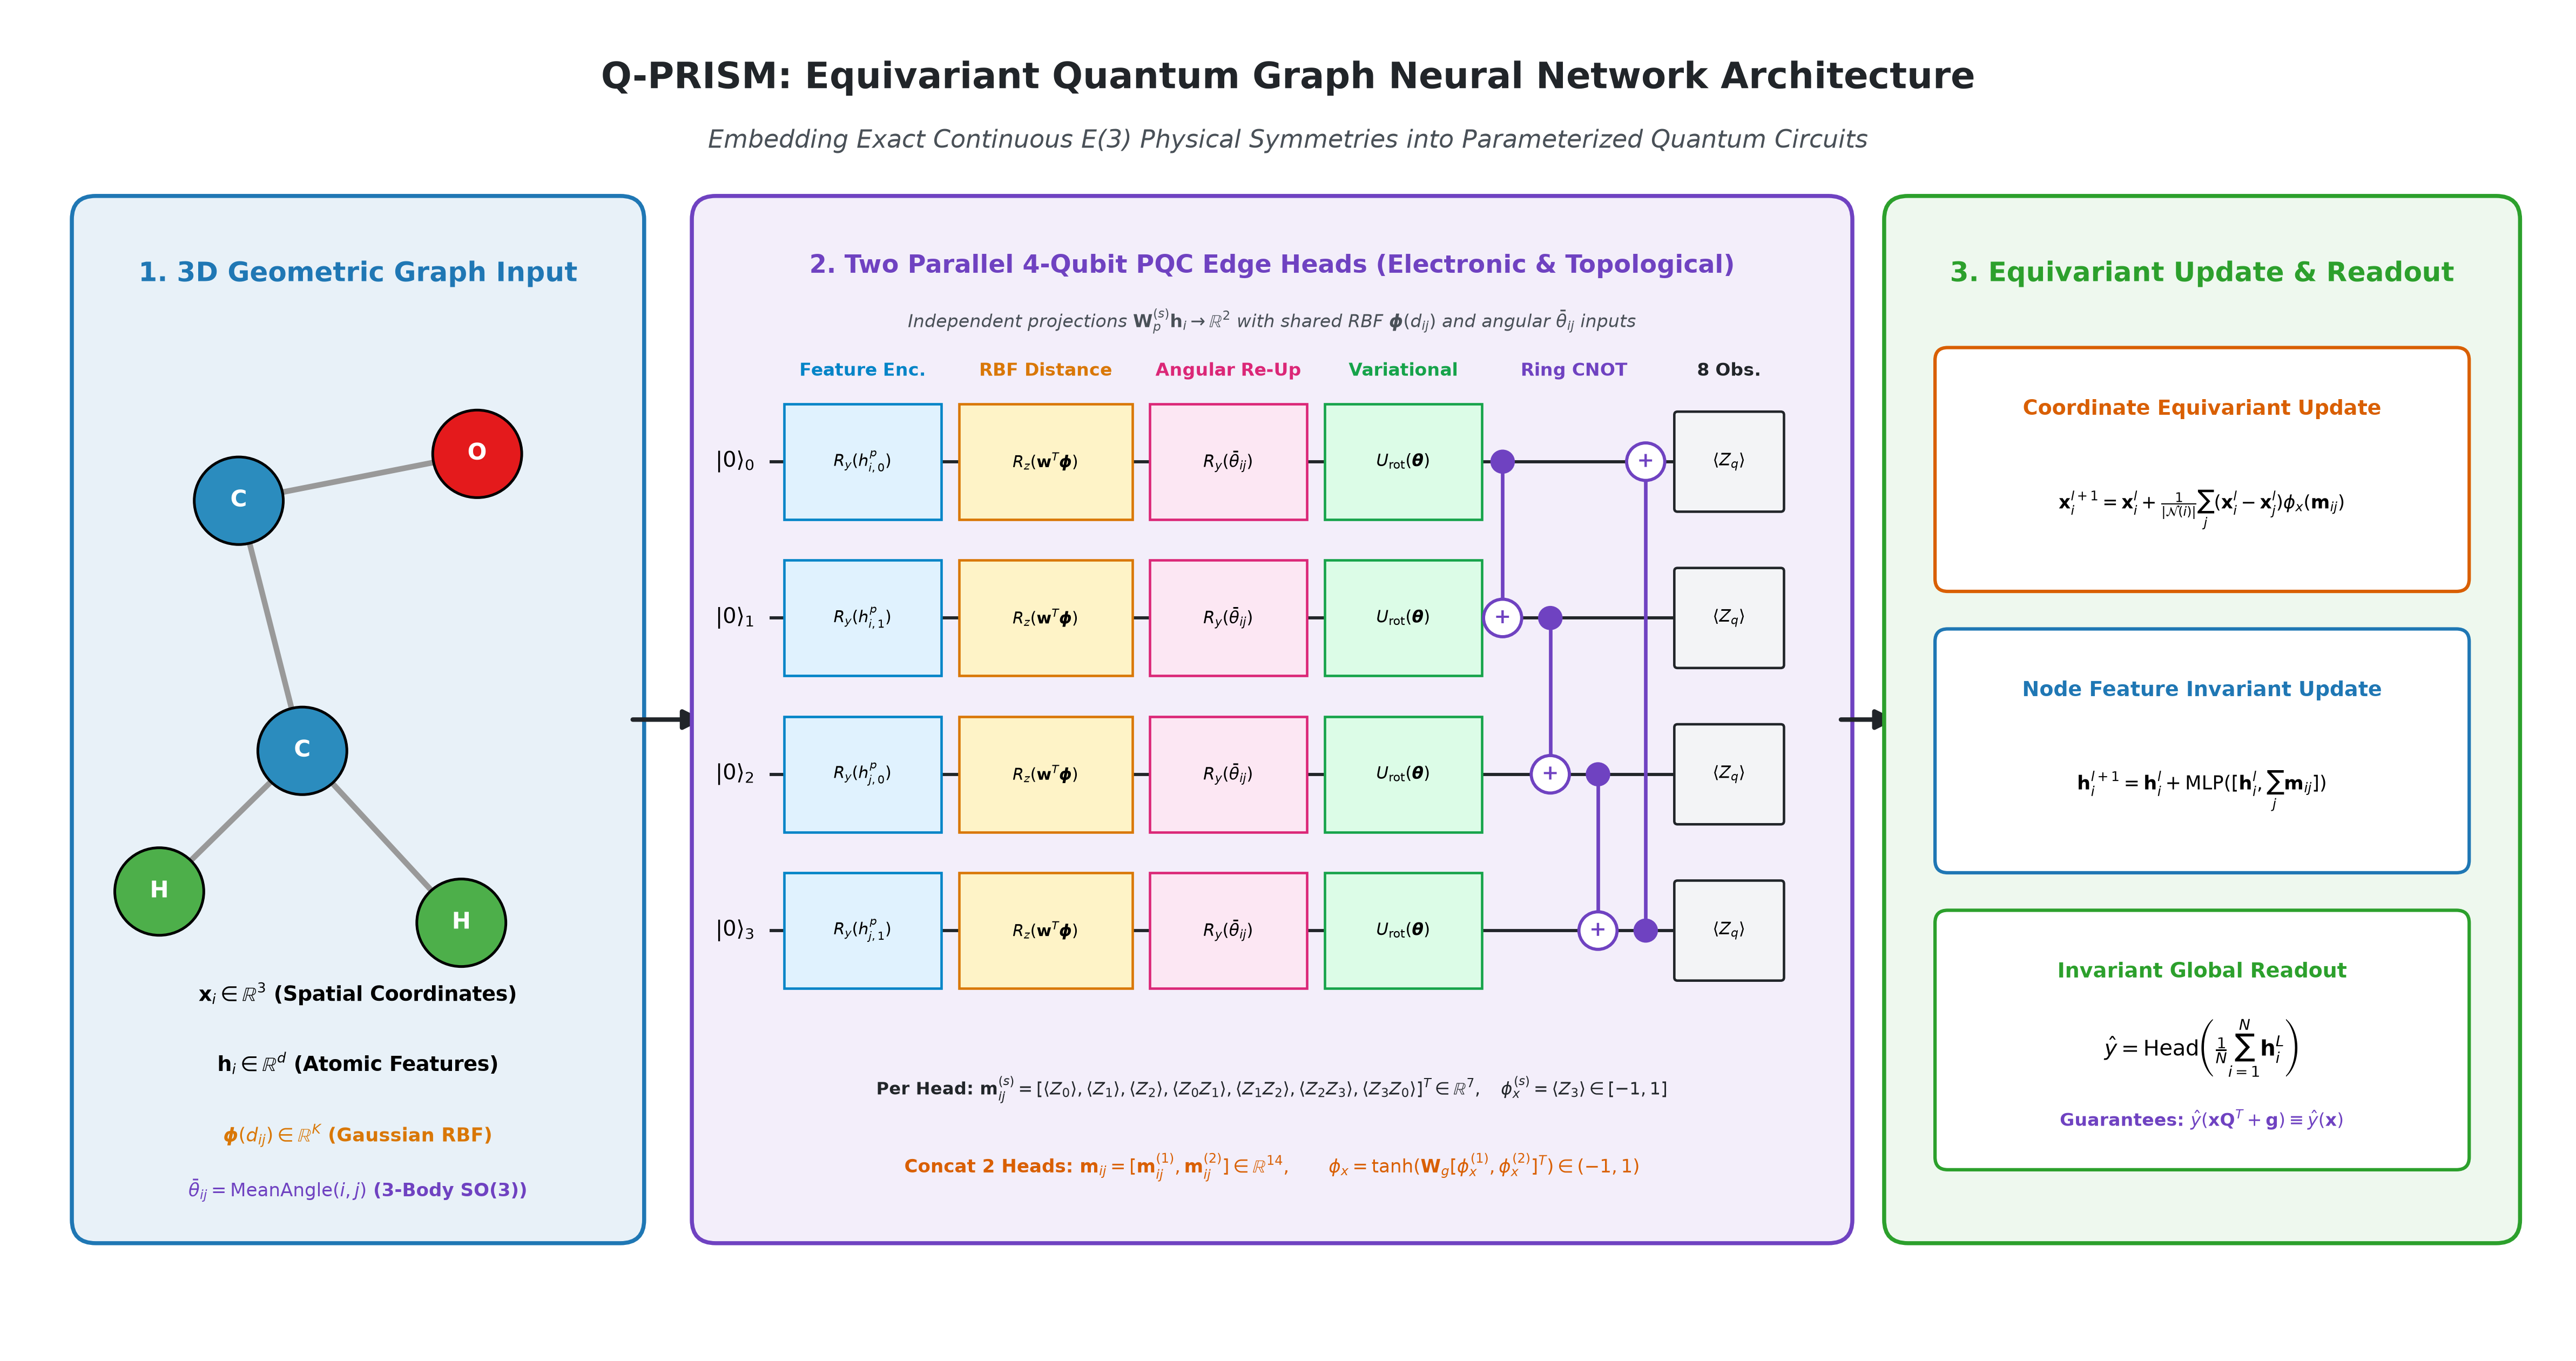
\includegraphics[width=\textwidth]{figures/figure_architecture.png}
    \caption{\textbf{Kiến trúc Q-PRISM:} (1) Đồ thị phân tử 3D đầu vào với các đặc trưng khoảng cách RBF bất biến $\boldsymbol{\phi}(d_{ij})$ và các góc liên kết bất biến $\mathrm{SO}(3)$ $\bar{\theta}_{ij}$. (2) Hai nhánh PQC 4-qubit song song (Điện tử \& Tô-pô) với kỹ thuật tải lại khoảng cách RBF đa tần số, mã hóa góc, các phép quay biến phân, và vướng víu CNOT dạng vòng. (3) Đọc 8 đại lượng quan sát trên mỗi nhánh: 4 phép đo đơn qubit $\langle Z_q \rangle$ + 4 tương quan tử $\langle Z_i Z_j \rangle$. (4) Cập nhật tọa độ tương biến có cổng kích hoạt $\tanh$ và truyền thông điệp đặc trưng bất biến tạo ra các dự đoán tính chất phân tử toàn cục.}
    \label{fig:architecture}
\end{figure*}

\subsection{Tích chập Cạnh Lượng tử}
\label{sec:quantum_edge}

Như minh họa trong Hình~\ref{fig:architecture}, giả sử một phân tử 3D được biểu diễn dưới dạng đồ thị $\mathcal{G} = (\mathcal{V}, \mathcal{E}, \mathbf{x}, \mathbf{h})$, trong đó mỗi nguyên tử $i \in \mathcal{V}$ có tọa độ không gian $\mathbf{x}_i \in \mathbb{R}^3$ và vector đặc trưng nguyên tử bất biến $\mathbf{h}_i \in \mathbb{R}^{d_{\mathrm{in}}}$. Các cạnh $(i, j) \in \mathcal{E}$ kết nối các cặp nguyên tử tương tác trong bán kính ngưỡng, xác định tập láng giềng $\mathcal{N}(i) = \{j : (i, j) \in \mathcal{E}\}$. Bình phương khoảng cách Euclid là:
\begin{equation}
    d_{ij} = \|\mathbf{x}_i - \mathbf{x}_j\|^2 \in \mathbb{R}_{\ge 0}
\end{equation}

\paragraph{Khai triển Khoảng cách RBF Gaussian.}
Thay vì mã hóa khoảng cách thô qua một trọng số vô hướng đơn lẻ $w_d^{(l)} \cdot d_{ij}$, chúng tôi khai triển khoảng cách vào một hệ cơ sở xuyên tâm Gaussian đa tần số~\cite{schütt2017schnetcontinuousfilterconvolutionalneural}:
\begin{equation}
    \phi_k(d_{ij}) = \exp\left(-\gamma_k (d_{ij} - \mu_k)^2\right), \quad k = 1, \ldots, K
    \label{eq:rbf}
\end{equation}
trong đó $\mu_k$ là các tâm cách đều nhau trong $[0, 10]$~\AA$^2$ và $\gamma_k$ là các độ rộng nghịch đảo học được. Dưới phân tích Fourier của kỹ thuật tải lại dữ liệu~\cite{Perez-Salinas:2019pjx, Schuld:2020enb}, điều này biến PQC thành một bộ xấp xỉ Fourier cắt cụt $K$ số hạng cho các mặt thế năng phân tử.

Mỗi qubit nhận một pha có trọng số theo từng tầng, từng qubit:
\begin{equation}
    R_z\!\left(\sum_{k=1}^K w_{d,q,k}^{(l)} \cdot \phi_k(d_{ij})\right), \quad q = 0, \ldots, 3
\end{equation}

\paragraph{Thiết kế Đa nhánh.}
Tuân theo các thiết kế chú ý đa đầu (multi-head attention), chúng tôi sử dụng hai nhánh PQC song song (\textit{Điện tử} và \textit{Tô-pô}). Mỗi nhánh sử dụng một phép chiếu đặc trưng độc lập $\mathbf{W}_p^{(s)}: \mathbb{R}^{d_{\mathrm{hidden}}} \to \mathbb{R}^2$ để điều hướng các không gian con đặc trưng riêng biệt vào mạch lượng tử tương ứng:
\begin{equation}
    \mathbf{h}_i^{p,(s)} = \mathbf{W}_p^{(s)} \mathbf{h}_i, \quad s \in \{1, 2\}
\end{equation}
Cả hai nhánh cùng chia sẻ các đặc trưng khoảng cách RBF và góc đầu vào nhưng xử lý chúng qua các tập tham số PQC độc lập.

\paragraph{Mạch Lượng tử Tham số hóa 4-Qubit.}
Đối với mỗi nhánh $s \in \{1, 2\}$ và cạnh có hướng $(i, j)$, vector đầu vào cạnh $\mathbf{u}_{ij}^{(s)} = [\mathbf{h}_i^{p,(s)\top}, \mathbf{h}_j^{p,(s)\top}, \boldsymbol{\phi}(d_{ij})^\top, \bar{\theta}_{ij}]^\top \in \mathbb{R}^{4+K+1}$ được xử lý bởi một mạch 4-qubit khởi tạo ở $|0\rangle^{\otimes 4}$. Như được phác thảo trong Hình~\ref{fig:architecture}(2), trạng thái tiến triển qua $L$ tầng biến phân thông qua phép hợp thành toán tử theo thứ tự thời gian, $|\psi_{ij}^{(s)}\rangle = \left(\prod_{l=L}^1 U^{(l)}(\mathbf{u}_{ij}^{(s)}, \boldsymbol{\theta}_l)\right) |0\rangle^{\otimes 4}$. Mỗi tầng biến phân $U^{(l)}$ hợp thành các phép đưa pha đơn qubit đa trục với một vòng vướng víu tuần hoàn:
\begin{align}
    U^{(l)}(\mathbf{u}_{ij}^{(s)}, \boldsymbol{\theta}_l) &= \mathcal{W}_{\mathrm{ring}} \bigotimes_{q=0}^3 \Big[ R_{ZYX}(\boldsymbol{\theta}_{l,q}) \, R_y(\bar{\theta}_{ij}) \nonumber \\
    &\quad \cdot R_z\!\left(\sum_{k=1}^K w_{d,q,k}^{(l)} \phi_k(d_{ij})\right) R_y(\tilde{h}_{ij,q}^{(s)}) \Big]
    \label{eq:layer_unitary}
\end{align}
trong đó các phép toán được tính toán theo thứ tự thời gian từ phải sang trái. Tại đây, $\tilde{\mathbf{h}}_{ij}^{(s)} = [\mathbf{h}_i^{p,(s)\top}, \mathbf{h}_j^{p,(s)\top}]^\top \in \mathbb{R}^4$ đưa các đặc trưng nguyên tử đã chiếu vào pha Pauli-$Y$ ban đầu trên qubit $q \in \{0, \dots, 3\}$; vector RBF Gaussian $K$-kênh $\boldsymbol{\phi}(d_{ij})$ được chiếu tuyến tính qua các trọng số huấn luyện được $\mathbf{w}_{d,q}^{(l)} \in \mathbb{R}^K$ vào pha Pauli-$Z$, đưa vào một hệ cơ sở khoảng cách Fourier cắt cụt; $\bar{\theta}_{ij}$ đưa góc liên kết trung bình bất biến $\mathrm{O}(3)$ vào phép quay Pauli-$Y$ thứ hai; $R_{ZYX}(\boldsymbol{\theta}_{l,q}) = R_z(\theta_{l,q,2}) R_y(\theta_{l,q,1}) R_x(\theta_{l,q,0})$ cung cấp phép quay Euler đơn qubit phổ quát với 3 tham số huấn luyện được trên mỗi qubit ($12$ tham số trên mỗi tầng); và $\mathcal{W}_{\mathrm{ring}} = \prod_{q=0}^3 \mathrm{CX}_{q \to (q+1)\bmod 4}$ luân chuyển thông tin pha lượng tử qua thanh ghi 4-qubit ($\mathrm{CX}_{c \to t}$ ký hiệu cổng controlled-NOT với qubit điều khiển $c$ và qubit đích $t$).

Phương trình~(\ref{eq:layer_unitary}) làm cho cơ chế khử lượng tử hóa trở nên minh bạch về mặt toán học: toàn bộ các kênh dữ liệu vật lý (loại nguyên tử, khoảng cách giữa các nguyên tử, và các góc 3 vật thể) đều được đóng gói chặt chẽ vào các phép quay pha đơn qubit cục bộ, xác nhận rằng việc tải lại dữ liệu vốn dĩ xây dựng các chuỗi Fourier đa kênh độc lập trước khi $\mathcal{W}_{\mathrm{ring}}$ ghép nối chúng.

\paragraph{Mã hóa Góc Bất biến SO(3) cho Tương tác 3 Vật thể.}
Đối với mỗi cạnh $(i, j)$, chúng tôi tính góc liên kết trung bình $\bar{\theta}_{ij}$ qua toàn bộ các nguyên tử thứ ba $k \in \mathcal{N}(i), k \neq j$ bằng các phép toán vector hóa $O(E)$:
\begin{align}
    \bar{\cos}_{ij} &= \frac{\hat{\mathbf{r}}_{ij} \cdot \sum_{k \in \mathcal{N}(i)} \hat{\mathbf{r}}_{ik} - 1}{\deg(i) - 1}, \label{eq:angle} \\
    \bar{\theta}_{ij} &= \arccos\!\left(\mathrm{clamp}(\bar{\cos}_{ij}, -1, 1)\right) \nonumber
\end{align}
trong đó $\hat{\mathbf{r}}_{ij} = (\mathbf{x}_j - \mathbf{x}_i) / \|\mathbf{x}_j - \mathbf{x}_i\|$. Đối với các nguyên tử đơn hóa trị ($\deg(i) = 1$), mẫu số trong Phương trình~(\ref{eq:angle}) được giới hạn về $1$, mang lại $\bar{\theta}_{ij} = \pi/2$ như một giá trị mặc định trung tính. Đại lượng này bất biến tuyệt đối $\mathrm{O}(3)$ vì $\cos \theta_{ijk} = \hat{\mathbf{r}}_{ij} \cdot \hat{\mathbf{r}}_{ik}$ chỉ phụ thuộc vào tích vô hướng của các vector tương đối: $(\mathbf{Q}\hat{\mathbf{r}}_{ij})^\top (\mathbf{Q}\hat{\mathbf{r}}_{ik}) = \hat{\mathbf{r}}_{ij}^\top \mathbf{Q}^\top \mathbf{Q} \hat{\mathbf{r}}_{ik} = \hat{\mathbf{r}}_{ij}^\top \hat{\mathbf{r}}_{ik}$.

\paragraph{Sự Thoái hóa Góc của Phép Gom cụm Trung bình.}
Phép lấy góc trung bình có thể ánh xạ các môi trường phối trí khác biệt về các giá trị vô hướng tương tự nhau (ví dụ: carbon sp$^3$ và sp$^2$ chỉ chênh lệch nhau $\sim 10^\circ$). Trong thực tế, các kênh embedding nút và khoảng cách RBF cung cấp đầy đủ thông tin bổ trợ để phân biệt rõ các phân tử hữu cơ trong QM9; việc mở rộng sang các hệ hóa học có phối trí đa dạng (như phức chất kim loại chuyển tiếp) đòi hỏi phép khai triển góc theo từng bộ ba nguyên tử~\cite{klicperaFastUncertaintyAwareDirectional2020, klicperaGemNetUniversalDirectional2021} (xem Hạn chế 2, SM~H).

\paragraph{Giá trị Đọc qua Tương quan tử Vướng víu.}
Mỗi nhánh sinh ra 8 đại lượng quan sát từ trạng thái đầu ra $|\psi_{ij}^{(s)}\rangle$: 4 kỳ vọng đơn qubit $\langle Z_q \rangle_{ij}^{(s)}$ và 4 tương quan tử dạng vòng $\langle Z_q Z_{(q+1)\bmod 4} \rangle_{ij}^{(s)}$ với $q \in \{0, 1, 2, 3\}$. 8 đại lượng quan sát này được phân chia thành các kênh tọa độ và đặc trưng:
\begin{align}
    \mathbf{m}_{ij}^{(s)} &= \big[\langle Z_0 \rangle, \langle Z_1 \rangle, \langle Z_2 \rangle, \nonumber \\
    &\quad \langle Z_0 Z_1 \rangle, \langle Z_1 Z_2 \rangle, \langle Z_2 Z_3 \rangle, \langle Z_3 Z_0 \rangle\big]^\top \in \mathbb{R}^7, \\
    \phi_x^{(s)} &= \langle Z_3 \rangle_{ij}^{(s)} \in [-1, 1].
\end{align}
Qubit 3 được chỉ định làm đại lượng quan sát cập nhật tọa độ vì nó nằm xa nhất so với các qubit mã hóa đặc trưng (0, 1) trong tô pô CNOT dạng vòng, nhờ đó $\phi_x^{(s)}$ mang tín hiệu đã qua xử lý vướng víu thay vì các góc quay đầu vào thô.

Thông điệp của hai nhánh được ghép nối lại: $\mathbf{m}_{ij} = [\mathbf{m}_{ij}^{(1)}, \mathbf{m}_{ij}^{(2)}] \in \mathbb{R}^{14}$.

\subsection{Truyền Thông điệp Tương biến}
\label{sec:message_passing}

Các đại lượng quan sát tọa độ theo từng nhánh $\phi_x^{(1)}, \phi_x^{(2)}$ từ Mục~\ref{sec:quantum_edge} được kết hợp thành một đại lượng vô hướng có cổng kích hoạt thông qua hàm $\tanh$, giới hạn mỗi bước cập nhật tọa độ trong khoảng $(-1, 1)$:
\begin{equation}
    \phi_x(\mathbf{m}_{ij}) = \tanh\!\left(\mathbf{W}_g \left[\phi_x^{(1)}, \phi_x^{(2)}\right]^T\right) \in (-1, 1)
\end{equation}
\begin{equation}
    \mathbf{x}_i^{l+1} = \mathbf{x}_i^l + \frac{1}{|\mathcal{N}(i)|} \sum_{j \in \mathcal{N}(i)} (\mathbf{x}_i^l - \mathbf{x}_j^l) \cdot \phi_x(\mathbf{m}_{ij})
    \label{eq:coord_update}
\end{equation}

\paragraph{Truyền thông điệp Đặc trưng Bất biến.}
Các thông điệp cạnh được tổng hợp trên từng nút và kết hợp với các đặc trưng hiện tại qua một bước cập nhật MLP phần dư:
\begin{align}
    \mathbf{m}_i &= \sum_{j \in \mathcal{N}(i)} \mathbf{m}_{ij} \\
    \mathbf{h}_i^{l+1} &= \mathbf{h}_i^l + \mathrm{MLP}\left([\mathbf{h}_i^l, \mathbf{m}_i]\right)
    \label{eq:feat_update}
\end{align}

\subsection{Khử Lượng tử hóa Cổ điển: PRISM}
\label{sec:periodic_egnn}

Để kiểm tra xem hiệu năng của PQC bắt nguồn từ các tính chất cơ học lượng tử hay từ năng lực biểu diễn lượng giác cổ điển, chúng tôi xây dựng các mô hình đại diện cổ điển tương thích cấu trúc theo khuôn khổ khử lượng tử hóa thực nghiệm~\cite{Tang:2018lmw, Schreiber:2022roq, pegg2026isoqgnn}.
Chúng tôi sử dụng thuật ngữ ``khử lượng tử hóa'' theo nghĩa gợi mở, thực nghiệm của Schreiber et al.~\cite{Schreiber:2022roq}: xây dựng một mô hình cổ điển với lớp giả thuyết tương đồng về mặt cấu trúc và chứng minh hiệu năng tương đương hoặc vượt trội (xem SM~D để biết thêm thảo luận chi tiết về thuật ngữ, sự bất đối xứng số chiều, và lựa chọn hàm kích hoạt).

\paragraph{Bản Song sinh Cổ điển ($\tanh$-MLP).}
Bản song sinh cổ điển tiêu chuẩn sử dụng mạng MLP hai tầng với các hàm kích hoạt thuộc họ sigmoid:
\begin{equation}
    \mathbf{o}_{ij}^{(s)} = \tanh\left(\mathbf{W}_2 \operatorname{SiLU}(\mathbf{W}_1 \mathbf{u}_{ij}^{(s)} + \mathbf{b}_1)\right)
\end{equation}
trong đó $\mathbf{W}_1 \in \mathbb{R}^{4 \times 13}$ và $\mathbf{W}_2 \in \mathbb{R}^{8 \times 4}$ (không có độ lệch bias). Ngân sách tham số huấn luyện được trên mỗi nhánh chính xác là $4 \times (13 + 1) + 4 \times 8 = 88$, khớp hoàn toàn với 88 tham số của PQC 4-qubit ($24$ góc quay $+ 64$ trọng số tải lại khoảng cách) tạo nên sự tương đương chính xác $2{,}527$ tham số trên toàn mô hình.

\paragraph{PRISM (Bản Song sinh Tuần hoàn SIREN).}
Để khắc phục giới hạn biểu diễn của hàm kích hoạt đơn điệu ở mức ngân sách tham số thấp~\cite{rahaman2019spectral, sitzmann2020siren}, chúng tôi thay thế hàm kích hoạt đơn điệu bằng phi tuyến hình sin tuần hoàn với phép khởi tạo SIREN~\cite{sitzmann2020siren}:
\begin{equation}
    \mathbf{o}_{ij}^{(s)} = \tanh\left(\mathbf{W}_2 \sin\left(\omega_0 (\mathbf{W}_1 \mathbf{u}_{ij}^{(s)} + \mathbf{b}_1)\right)\right)
\end{equation}
với siêu tham số tần số $\omega_0 = 30.0$ được cố định \textit{a priori} theo Sitzmann et al.~\cite{sitzmann2020siren}. Một đợt quét lưới 9 điểm mở rộng trên $\omega_0 \in [1, 100]$ (10 hạt giống, SM~D, Bảng~S5, Hình~S5) khẳng định rằng ưu thế tuần hoàn đặc biệt vững chắc trên các tần số, với dải cộng hưởng vật lý tối ưu xuất hiện tại $\omega_0 \approx 50$ (mang lại mức giảm sai số $-38.9\%$ so với Bản song sinh Cổ điển trên Gap).
Theo Sitzmann et al.~\cite{sitzmann2020siren}, các trọng số được khởi tạo như sau:
\begin{equation}
    \mathbf{W}_1 \sim \mathcal{U}\left(-\frac{1}{d_{\mathrm{edge}}}, \frac{1}{d_{\mathrm{edge}}}\right), \quad \mathbf{W}_2 \sim \mathcal{U}\left(-\frac{\sqrt{6/d_h}}{\omega_0}, \frac{\sqrt{6/d_h}}{\omega_0}\right)
\end{equation}
trong đó $d_{\mathrm{edge}} = 13$ và $d_h = 4$.
Điều này đảm bảo sự lan truyền phương sai đồng đều qua các hàm kích hoạt tuần hoàn, bảo toàn các gradient góc dao động mà không gặp hiện tượng bão hòa số học. Số lượng tham số huấn luyện được duy trì chính xác ở mức $2{,}527$ tham số.

\paragraph{Bản Song sinh Đặc trưng Fourier Ngẫu nhiên (RFF).}
Như một đường cơ sở thay thế, chúng tôi triển khai Đặc trưng Fourier Ngẫu nhiên (RFF) theo Tancik et al.~\cite{tancik2020fourier}:
$\gamma(\mathbf{u}) = [\cos(2\pi \mathbf{B}\mathbf{u}), \sin(2\pi \mathbf{B}\mathbf{u})]^T$, trong đó $\mathbf{B} \in \mathbb{R}^{13 \times 4}$ là ma trận ngẫu nhiên Gaussian cố định ($\sigma = 10.0$), theo sau là một phép chiếu tuyến tính khớp $2{,}515$ tham số ($\Delta = -12$).

Vì tất cả các đầu vào $\mathbf{u}_{ij}^{(s)}$ đều bất biến tuyệt đối $\mathrm{O}(3)$, Định lý~\ref{thm:equivariance} áp dụng tương tự cho PRISM, Bản song sinh Cổ điển ($\tanh$), và các bản song sinh Đặc trưng Fourier, bảo đảm tính tương biến $\mathrm{E}(3)$ chính xác ở cấp độ máy cho mọi biến thể cổ điển.

\subsection{Bảo đảm Lý thuyết}
\label{sec:theory}

\begin{theorem}[Tính Tương biến $\mathrm{E}(3)$ của Tầng Q-PRISM]
\label{thm:equivariance}
Ký hiệu $\mathcal{T}_{\mathbf{Q}, \mathbf{g}}(\mathbf{x}) = \mathbf{x} \mathbf{Q}^T + \mathbf{g}$ là một phép biến đổi Euclid liên tục bất kỳ với phép quay/phản xạ $\mathbf{Q} \in \mathrm{O}(3)$ và phép tịnh tiến $\mathbf{g} \in \mathbb{R}^3$.\footnote{Chúng tôi áp dụng quy ước vector hàng xuyên suốt: các tọa độ được lưu trữ dưới dạng $\mathbf{x}_i \in \mathbb{R}^{1 \times 3}$ (vector hàng), do đó phép biến đổi là $\mathbf{x} \mathbf{Q}^T + \mathbf{g}$ thay vì $\mathbf{Q}\mathbf{x} + \mathbf{g}$. Điều này khớp với bố cục batch-of-row-vectors mặc định của PyTorch.} Khi đó đối với tầng Q-PRISM được định nghĩa trong các Phương trình~(\ref{eq:coord_update}--\ref{eq:feat_update}):
\begin{align}
    \mathbf{h}_i^{l+1}(\mathcal{T}_{\mathbf{Q}, \mathbf{g}}(\mathbf{x}), \mathbf{h}) &= \mathbf{h}_i^{l+1}(\mathbf{x}, \mathbf{h}) \quad (\text{Tính Bất biến}) \\
    \mathbf{x}_i^{l+1}(\mathcal{T}_{\mathbf{Q}, \mathbf{g}}(\mathbf{x}), \mathbf{h}) &= \mathcal{T}_{\mathbf{Q}, \mathbf{g}}(\mathbf{x}_i^{l+1}(\mathbf{x}, \mathbf{h})) \quad (\text{Tính Tương biến})
\end{align}
\end{theorem}

Chứng minh suy ra từ tính bất biến $\mathrm{O}(3)$ của toàn bộ các đầu vào PQC ($d_{ij}$, $\bar{\theta}_{ij}$, $\mathbf{h}_i$) và cấu trúc tương biến của phép cập nhật tọa độ (Phương trình~\ref{eq:coord_update}); xem SM~C để biết toàn bộ các bước suy dẫn. Kiểm tra số học với các phép quay $\mathrm{O}(3)$ ngẫu nhiên xác nhận sai số tương biến $\le 2.38 \times 10^{-7}$. Mã giả thuật toán được cung cấp trong SM~C.

\section{Đánh giá Thực nghiệm}
\label{sec:experiments}

\subsection{Thiết lập Chuẩn Thực nghiệm}

Chúng tôi đánh giá Q-PRISM trên \textbf{tập dữ liệu chuẩn QM9} \cite{ramakrishnan2014quantum}, bao gồm $130{,}831$ phân tử hữu cơ nhỏ với các tính chất điện tử lượng tử được tính toán ở mức DFT B3LYP/6-31G(2df,p).
Chúng tôi thực hiện đánh giá trên \textbf{6 mục tiêu vật lý} sử dụng \textbf{5 hạt giống ngẫu nhiên độc lập} ($42$--$46$) trên $N = 1{,}000$ phân tử huấn luyện và $500$ phân tử kiểm tra.
Chúng tôi lựa chọn các mục tiêu bao quát ba cơ chế vật lý phân biệt: các tính chất điện tử nồng độ (intensive electronic properties: HOMO, LUMO, Gap) thăm dò sự xen phủ orbital góc đóng vai trò trung tâm trong giả thuyết thiên kiến phổ; các tính chất tĩnh điện dung lượng (extensive electrostatic properties: mômen lưỡng cực $\mu$, độ phân cực $\alpha$) kiểm tra sự phân bố điện tích phụ thuộc tọa độ; và năng lượng nhiệt động dung lượng ($U_0$). Chúng tôi lưu ý rằng năng lượng LUMO KS-DFT, không giống như năng lượng HOMO (vốn xấp xỉ thế ion hóa qua định lý Koopmans tương đương trong Kohn-Sham), thiếu cách diễn giải vật lý chặt chẽ và phụ thuộc nhiều vào hệ cơ sở; các kết quả LUMO nên được hiểu cùng lưu ý này. Các tính chất QM9 còn lại ($U$, $H$, và $G$) dẫn xuất tuyến tính từ $U_0$ qua các hiệu chỉnh nhiệt và entropy, khiến các so sánh riêng biệt trở nên dư thừa. Các tính chất dao động ($\text{ZPVE}$ và $C_v$) nằm ngoài dung lượng của các mô hình thu gọn $\sim 2{,}500$ tham số.
Phân chia $1{,}000 / 500$ (tỷ lệ 2:1) đại diện cho một giao thức chuẩn cho việc đánh giá hóa học trong chế độ dữ liệu ít, cung cấp đủ năng lực thống kê cho các so sánh theo cặp trong khi vẫn duy trì tính khả thi tính toán trên 8 mô hình và các đợt quét đa hạt giống.
Toàn bộ các siêu tham số huấn luyện (bộ tối ưu hóa, tốc độ học, bộ điều chỉnh tốc độ học scheduler, kích thước batch, dừng sớm early stopping, và tài nguyên tính toán) được cung cấp trong SM~A, Bảng~S1.
Tất cả các thí nghiệm sử dụng 5 hạt giống ngẫu nhiên độc lập kiểm soát cả việc khởi tạo lẫn phân chia dữ liệu; phân tích triệt tiêu 20 hạt giống (Mục~\ref{sec:mechanism}) khẳng định tính vững chắc. Chi tiết thống kê (giao thức hạt giống, phân tích năng lực kiểm định, kiểm định Wilcoxon) được trình bày trong SM~B.

Chúng tôi đánh giá trên một hệ phân cấp 8 mô hình: (i) \textit{Bản song sinh Cổ điển} ($\tanh$-MLP, $2{,}527$\,p), (ii) \textit{PRISM} (SIREN, $2{,}527$\,p), (iii) \textit{Bản song sinh RFF} ($2{,}515$\,p), (iv--v) SchNet ($2{,}473$\,p) và PaiNN ($2{,}721$\,p), (vi--vii) EGNN đồng tham số và tiêu chuẩn, và (viii) mô hình kiểm chứng GNN không tương biến.

\begin{table*}[t]
\centering
\footnotesize
\setlength{\tabcolsep}{2.5pt}
\caption{\textbf{Đối chuẩn QM9 Đa Mục tiêu trên 8 Mô hình với các Bản Song sinh Lượng giác Khử lượng tử hóa và các Mô hình Đường cơ sở SOTA} ($N = 1{,}000$, Trung bình $\pm$ Độ lệch chuẩn trên 5 Hạt giống). Kết quả tốt nhất mỗi dòng được in \textbf{đậm}. Để tham khảo, ngưỡng độ chính xác hóa học là $0.043$\,eV ($1$\,kcal/mol); toàn bộ các mô hình đều hoạt động ở phía trên ngưỡng này trong chế độ ràng buộc tham số. Mức ý nghĩa thống kê của PRISM (SIREN) so với Bản song sinh Cổ điển ($\tanh$) dưới hiệu chỉnh đa giả thuyết Benjamini-Hochberg FDR ($m = 48$ giả thuyết): $^{\dagger}q < 0.05$, $^{\dagger\dagger}q < 0.01$. Mức ý nghĩa của Q-PRISM so với Bản song sinh Cổ điển ($\tanh$): $^*p < 0.05$, $^{**}p < 0.01$ (kiểm định $t$ theo cặp chưa hiệu chỉnh; xem Bảng~\ref{tab:full_48_fdr} trong Phụ lục~\ref{sec:appendix_fdr} để biết báo cáo FDR đầy đủ).}
\label{tab:main_results}
\resizebox{\textwidth}{!}{%
\begin{tabular}{llccccccccc}
\toprule
\textbf{Tính chất Mục tiêu} & \textbf{Đơn vị} & \textbf{Loại} & \textbf{Q-PRISM} & \textbf{PRISM} & \textbf{Song sinh Lượng giác} & \textbf{Song sinh Cổ điển} & \textbf{SchNet} & \textbf{PaiNN} & \textbf{EGNN-PM} & \textbf{EGNN Chuẩn} \\
 & & & (Của chúng tôi: PQC) & \textbf{(Của chúng tôi: SIREN)} & (Fourier) & ($\tanh$-MLP) & & & & \\
 & & & $2{,}527$\,p & $2{,}527$\,p & $2{,}515$\,p & $2{,}527$\,p & $2{,}473$\,p & $2{,}721$\,p & $2{,}497$\,p & $4{,}289$\,p \\
\midrule
\multicolumn{11}{l}{\textit{Tính chất Orbital Điện tử (Nồng độ)}} \\
\quad HOMO ($\epsilon_{\mathrm{H}}$) & eV & Điện tử & $0.303 \pm 0.014$ & $\mathbf{0.269 \pm 0.015}^{\dagger}$ & $0.424 \pm 0.016$ & $0.344 \pm 0.045$ & $0.381 \pm 0.025$ & $0.283 \pm 0.030$ & $0.365 \pm 0.020$ & $0.356 \pm 0.024$ \\
\quad LUMO ($\epsilon_{\mathrm{L}}$) & eV & Điện tử & $0.628 \pm 0.031^{**}$ & $0.479 \pm 0.015^{\dagger\dagger}$ & $0.775 \pm 0.030$ & $0.720 \pm 0.037$ & $0.692 \pm 0.023$ & $\mathbf{0.398 \pm 0.033}$ & $0.695 \pm 0.040$ & $0.693 \pm 0.024$ \\
\quad Gap ($\Delta\epsilon$) & eV & Điện tử & $0.721 \pm 0.055^{*}$ & $0.557 \pm 0.020^{\dagger\dagger}$ & $0.846 \pm 0.036$ & $0.806 \pm 0.041$ & $0.769 \pm 0.036$ & $\mathbf{0.470 \pm 0.069}$ & $0.769 \pm 0.047$ & $0.776 \pm 0.036$ \\
\midrule
\multicolumn{11}{l}{\textit{Tính chất Phân tử (Dung lượng)}} \\
\quad Lưỡng cực ($\mu$) & Debye & Dung lượng & $0.764 \pm 0.032^{*}$ & $\mathbf{0.711 \pm 0.020}^{\dagger}$ & $1.042 \pm 0.029$ & $0.904 \pm 0.088$ & $0.924 \pm 0.020$ & $0.819 \pm 0.098$ & $0.879 \pm 0.039$ & $0.851 \pm 0.057$ \\
\quad Độ phân cực ($\alpha$) & Bohr$^3$ & Dung lượng & $1.446 \pm 0.090$ & $\mathbf{1.415 \pm 0.088}^{\dagger}$ & $3.903 \pm 0.196$ & $1.841 \pm 0.226$ & $1.989 \pm 0.208$ & $3.446 \pm 0.257$ & $1.711 \pm 0.181$ & $1.419 \pm 0.058$ \\
\quad Nội năng ($U_0$) & eV & Dung lượng & $110.0 \pm 18.2$ & $130.6 \pm 29.3$ & $686.5 \pm 40.0$ & $101.1 \pm 16.7$ & $104.3 \pm 11.0$ & $446.0 \pm 25.1$ & $87.7 \pm 22.2$ & $\mathbf{69.5 \pm 12.3}$ \\
\midrule
\multicolumn{3}{l}{\textbf{Tham số Huấn luyện được}} & $\mathbf{2{,}527}$ & $\mathbf{2{,}527}$ & $2{,}515$ & $2{,}527$ & $2{,}473$ & $2{,}721$ & $2{,}497$ & $4{,}289$ \\
\bottomrule
\end{tabular}%
}
\end{table*}

\subsection{Kết quả Chính: Khử Lượng tử hóa qua PRISM}
\label{sec:periodic_results}

Bảng~\ref{tab:main_results} và Hình~\ref{fig:dequantization_bars} cung cấp một kiểm định trực tiếp đối với giả thuyết thiên kiến quy nạp lượng tử. Mạch PQC 4-qubit cho thấy MAE thấp hơn từ $10$--$16\%$ so với Bản song sinh Cổ điển trên các tính chất điện tử. Tuy nhiên, khi bản song sinh cổ điển được trang bị hàm kích hoạt tuần hoàn SIREN (\textbf{PRISM}, $2{,}527$\,p), lợi thế lượng tử biểu kiến hoàn toàn biến mất: PRISM vượt trội hơn Q-PRISM trên \textit{toàn bộ} các mục tiêu điện tử (HOMO: $0.269$ so với $0.303$\,eV, $q_{\mathrm{FDR}} = 0.002$; LUMO: $0.479$ so với $0.628$\,eV; Gap: $0.557$ so với $0.721$\,eV). PRISM cũng vượt trội hơn PaiNN trên 4 trong số 6 mục tiêu ở cùng mức ngân sách tham số, mặc dù các kênh vô hướng-vector kết hợp của PaiNN vẫn giữ ưu thế trên LUMO và Gap nơi thông tin vector định hướng đóng vai trò quan trọng. Bản song sinh RFF ($2{,}515$\,p) thất bại trên toàn bộ các mục tiêu, khẳng định rằng các tần số tuần hoàn \textit{được học} phù hợp với cấu trúc góc của mục tiêu, chứ không phải các hệ cơ sở tuần hoàn tùy ý, là yếu tố thúc đẩy sự cải thiện.
Trên $U_0$, PRISM kém hơn Bản song sinh Cổ điển ($130.6$ so với $101.1$\,eV, $p = 0.13$), khẳng định rằng ưu thế tuần hoàn mang tính đặc hiệu cho các tính chất điện tử phụ thuộc vào góc hơn là một sự gia tăng dung lượng chung chung.
Việc hiệu chỉnh đa giả thuyết thống kê toàn diện (Benjamini-Hochberg FDR, $m = 48$ giả thuyết) khẳng định ý nghĩa thống kê tại $q < 0.04$ cho 5 trong số 6 mục tiêu (Bảng~\ref{tab:full_48_fdr}, Phụ lục~\ref{sec:appendix_fdr}).

\begin{figure*}[t]
    \centering
    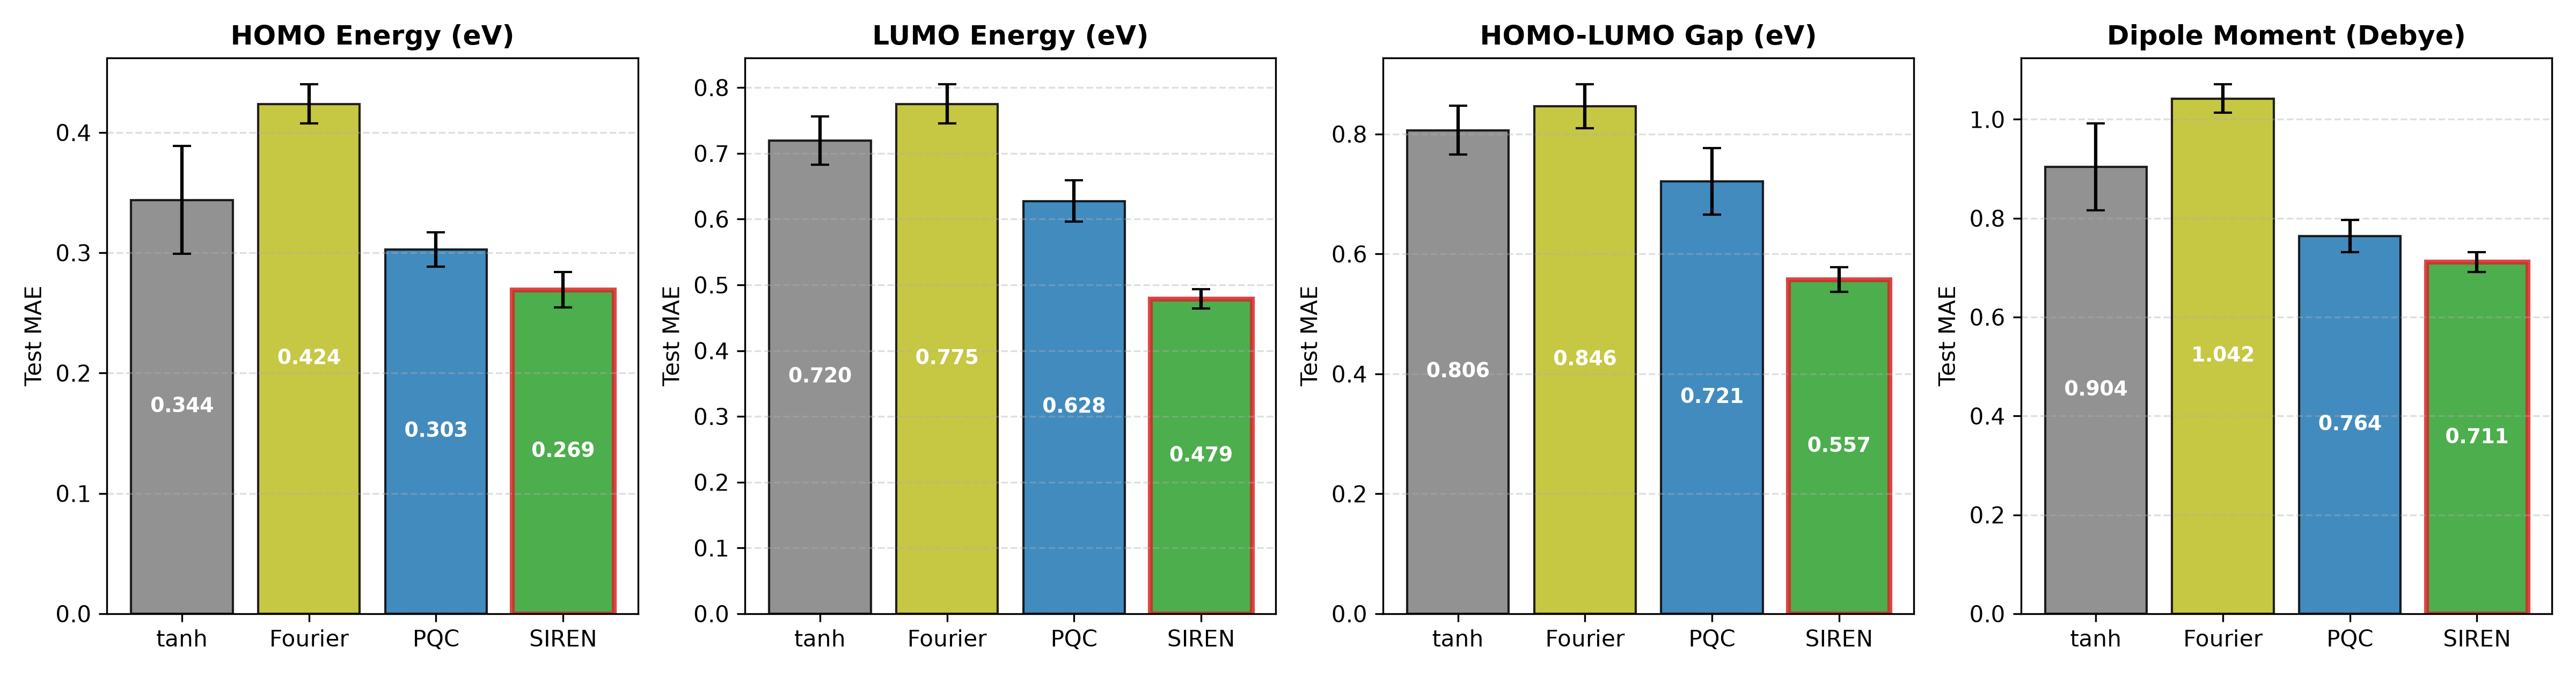
\includegraphics[width=0.95\textwidth]{figures/figure9_dequantization_comparison.png}
    \caption{\textbf{So sánh Khử lượng tử hóa trên các Mục tiêu Điện tử QM9 và Mômen Lưỡng cực:} MAE kiểm tra trên bốn mô hình cạnh cùng dung lượng ($2{,}527 \pm 12$ tham số mỗi mô hình): Bản song sinh Cổ điển ($\tanh$), Bản song sinh Đặc trưng Fourier Ngẫu nhiên (RFF), Q-PRISM (PQC 4-qubit), và PRISM (SIREN). Viền đỏ biểu thị mô hình đạt thành tích cao nhất trên từng mục tiêu. PRISM vượt trội hoàn toàn so với PQC và $\tanh$-MLP tiêu chuẩn trên cả bốn mục tiêu.}
    \label{fig:dequantization_bars}
\end{figure*}

\subsection{Cơ chế của Lợi thế Lượng tử}
\label{sec:mechanism}

Một phản biện tự nhiên là mạng MLP cổ điển với đầu ra $\tanh$ cũng sinh ra các đầu ra bị chặn tương tự $\in (-1, 1)$, có khả năng tái tạo bất kỳ thiên kiến quy nạp nào từ các đại lượng quan sát Pauli~\cite{bowles2024better}. Chúng tôi cô lập cơ chế hoạt động thông qua ba phân tích bổ trợ (phân tích đáp ứng hàm và mở rộng độ phức tạp mẫu trong SM~D và SM~E).

\paragraph{Triệt tiêu Vướng víu Đồng Kiến trúc.}
Theo Bowles et al.~\cite{bowles2024better}, chúng tôi xây dựng bốn mô hình ở mức khớp tham số nghiêm ngặt ($2{,}527$\,p) và đánh giá trên 20 hạt giống (Bảng~\ref{tab:iso_ablation}).

\begin{table*}[t]
\centering
\small
\caption{\textbf{Phân tích Triệt tiêu Đồng Dung lượng Bốn Bậc trên các Mục tiêu Điện tử QM9} ($N = 1{,}000$, 20 hạt giống, $d_{\min} = 0.47$). $d_{\min}$: kích thước hiệu ứng Cohen's $d$ tối thiểu có thể phát hiện được ở năng lực kiểm định 80\% với $n = 20$ quan sát theo cặp và $\alpha = 0.05$ (một phía). So sánh khớp tham số nhằm cô lập cơ chế của lợi thế lượng tử. Giá trị $p$ của kiểm định $t$ theo cặp: $^{*}p < 0.05$, $^{**}p < 0.01$, $^{***}p < 0.001$, so sánh giữa Vướng víu đối chiếu với Tách biệt và từng biến thể PQC so với mô hình cơ sở $\tanh$-MLP Cổ điển (dòng 3). EGNN Khớp Tham số báo cáo các giá trị 5 hạt giống từ Bảng~\ref{tab:main_results}. Lưu ý: Q-PRISM ($0.310$) và $\tanh$-MLP Cổ điển ($0.334$) khác biệt nhẹ so với Bảng~\ref{tab:main_results} do lấy trung bình trên 20 hạt giống so với 5 hạt giống với các tập khởi tạo ngẫu nhiên chồng lấn một phần nhưng phân biệt.}
\label{tab:iso_ablation}
\resizebox{0.95\textwidth}{!}{%
\begin{tabular}{llcccc}
\toprule
\textbf{Mô hình} & \textbf{Toán tử Cạnh} & \textbf{Số tham số} & \textbf{HOMO (eV)} & \textbf{LUMO (eV)} & \textbf{Gap (eV)} \\
\midrule
Q-PRISM (Của chúng tôi) & PQC Vướng víu & $2{,}527$ & $\mathbf{0.310 \pm 0.016}^{**\dagger}$ & $0.666 \pm 0.033^{***}$ & $0.740 \pm 0.047^{***}$ \\
Q-PRISM Tách biệt & PQC Không vướng víu & $2{,}527$ & $0.317 \pm 0.017^{**}$ & $\mathbf{0.656 \pm 0.035}^{***}$ & $\mathbf{0.719 \pm 0.046}^{***}$ \\
$\tanh$-MLP Cổ điển & Bị chặn Cổ điển & $2{,}527$ & $0.334 \pm 0.023$ & $0.747 \pm 0.029$ & $0.827 \pm 0.029$ \\
EGNN Khớp Tham số & SiLU Cổ điển & $2{,}497$ & $0.365 \pm 0.020$ & $0.695 \pm 0.040$ & $0.769 \pm 0.047$ \\
\bottomrule
\multicolumn{6}{l}{\footnotesize $\dagger$ Vướng víu so với Tách biệt: $p = 0.002$ (HOMO), $p = 0.33$ (LUMO), $p = 0.16$ (Gap).}
\end{tabular}%
}
\end{table*}

Sự vướng víu chỉ mang lại sự khác biệt có thể phát hiện được trên HOMO ($\Delta = 0.006$\,eV, $p = 0.002$, Cohen's $d = 0.85$), nhưng độ lớn tuyệt đối là không đáng kể trong thực tế ($2\%$ tương đối, nằm sâu trong ngưỡng độ chính xác hóa học). Trên LUMO ($p = 0.33$) và Gap ($p = 0.16$), sự vướng víu không mang lại bất kỳ sự cải thiện nào. Việc loại bỏ hoàn toàn sự vướng víu vẫn giúp PQC tách biệt vượt xa mô hình cổ điển $\tanh$-MLP (LUMO: $-12.2\%$, $p < 10^{-7}$; Gap: $-13.0\%$, $p < 10^{-8}$). Những dữ liệu này khẳng định rằng các phép quay lượng giác đơn qubit, chứ không phải sự vướng víu đa qubit, tạo ra sự khác biệt về hiệu năng.

\paragraph{Kích hoạt đối chiếu với Khởi tạo: Triệt tiêu Giai thừa.}
\label{sec:init_ablation}
Một thiết kế nhân tố $2 \times 2$ đan kết giữa các hàm kích hoạt $\{\sin, \mathrm{SiLU}/\tanh\}$ với các phép khởi tạo $\{\text{SIREN}, \text{Xavier}\}$ (10 hạt giống, Bảng~\ref{tab:init_ablation}) chỉ ra rằng hàm kích hoạt tuần hoàn $\sin$ là yếu tố chi phối chính (hiệu ứng chính cận biên ANOVA: $-0.16$ đến $-0.18$\,eV trên LUMO/Gap), với phép khởi tạo SIREN đóng góp vai trò thứ cấp ($-0.07$ đến $-0.09$\,eV). Sự kết hợp mang tính hiệp đồng rõ nét: không một yếu tố đơn lẻ nào có thể đạt đến hiệu năng đầy đủ của PRISM. Toàn bộ các khác biệt theo cặp giữa PRISM và các biến thể khác đều có ý nghĩa thống kê ($p < 0.002$, Cohen's $d > 2.0$).

\begin{table}[h]
\centering
\small
\caption{\textbf{Triệt tiêu Giai thừa $2 \times 2$: Hàm kích hoạt $\times$ Phép khởi tạo} ($N = 1{,}000$, 10 hạt giống). MAE kiểm tra (eV), trung bình $\pm$ độ lệch chuẩn. Toàn bộ bốn mô hình đều có chính xác $2{,}527$ tham số. Hàm kích hoạt tuần hoàn $\sin$ là yếu tố chi phối; khởi tạo SIREN đóng góp phần hiệp đồng thứ cấp. Toàn bộ các khác biệt theo cặp giữa PRISM và các biến thể khác đều có ý nghĩa thống kê ($p < 0.002$, Cohen's $d > 2.0$).}
\label{tab:init_ablation}
\resizebox{\columnwidth}{!}{%
\begin{tabular}{lcccc}
\toprule
\textbf{Mục tiêu} & \textbf{PRISM} & \textbf{Sin + Xavier} & \textbf{SiLU + SIREN} & \textbf{Song sinh Cổ điển} \\
 & (Sin + SIREN) & & (khởi tạo) & (SiLU + Tiêu chuẩn) \\
\midrule
HOMO & $\mathbf{0.272 \pm 0.014}$ & $0.357 \pm 0.025$ & $0.409 \pm 0.030$ & $0.343 \pm 0.041$ \\
LUMO & $\mathbf{0.494 \pm 0.031}$ & $0.666 \pm 0.023$ & $0.762 \pm 0.023$ & $0.727 \pm 0.034$ \\
Gap  & $\mathbf{0.540 \pm 0.030}$ & $0.740 \pm 0.056$ & $0.823 \pm 0.029$ & $0.815 \pm 0.035$ \\
\bottomrule
\end{tabular}%
}
\end{table}

\subsection{Mở rộng Dung lượng và Quy mô Tập Dữ liệu}
\label{sec:param_scaling}

\paragraph{Mở rộng Dung lượng qua Sáu Bậc Quy mô ($2.5\mathrm{k} \to 100\mathrm{k}+$ Tham số).}
Một câu hỏi then chốt là liệu ưu thế tuần hoàn có phải là hệ quả giả tạo do sự thiếu hụt tham số trong các mô hình thu gọn ($\sim 2{,}500$ tham số) hay không. Để kiểm chứng điều này, chúng tôi đánh giá PRISM, Bản song sinh Cổ điển, và PaiNN trên sáu bậc dung lượng: XS ($2{,}527$\,p), S ($4{,}911$\,p), M ($8{,}287$\,p), L ($16{,}959$\,p), XL ($29{,}599$\,p), và XXL ($100{,}127$\,p) trên 5 hạt giống độc lập đối với các mục tiêu điện tử QM9 (SM~E, Bảng~S8, Hình~S9). 
Không hề suy giảm khi dung lượng tăng lên, ưu thế tuần hoàn \textit{mở rộng một cách đơn điệu}: trên khe HOMO-LUMO, mức cải thiện tương đối của PRISM so với Bản song sinh Cổ điển tăng từ $+35.7\%$ ở mức XS ($0.518$ so với $0.806$\,eV, $p = 0.0009$) lên $+41.4\%$ ở mức M ($0.470$ so với $0.802$\,eV, $p = 0.0003$), đạt $\mathbf{+51.3\%}$ ở mức XXL ($0.370$ so với $0.761$\,eV, $p = 2.18 \times 10^{-5}$, $d$ của Cohen $= -10.21$). Trên HOMO, PRISM đạt $0.233$\,eV tiệm cận PaiNN ($0.210$\,eV), và trên LUMO đạt $0.265$\,eV ở quy mô $100\mathrm{k}$ tham số ($+50.6\%$ so với bản song sinh cổ điển, $p < 10^{-5}$, $d = -12.85$). Ở bậc XXL ($100\mathrm{k}+$ tham số), sai số của PRISM đạt trạng thái bão hòa quanh $\sim 0.370$\,eV trên Gap, phản ánh mức nhiễu mẫu nội tại của chế độ huấn luyện $N = 1{,}000$; tuy vậy, bản song sinh cổ điển bão hòa ở mức sai số cao hơn đáng kể ($\sim 0.761$\,eV), giúp ưu thế tuần hoàn duy trì trên $51\%$. Điều này xác nhận rằng các hàm kích hoạt tuần hoàn cung cấp một phần tử biểu diễn có khả năng mở rộng quy mô chứ không đơn thuần là một bộ điều chuẩn ở mức tham số thấp.

\paragraph{Đánh giá QM9 Toàn Quy mô ($N = 110{,}000$, 5 Hạt giống).}
Nhằm đảm bảo các phát hiện của chúng tôi không bị giới hạn trong chế độ dữ liệu khan hiếm ($N = 1{,}000$), chúng tôi đánh giá PRISM và Bản song sinh Cổ điển trên toàn bộ tập dữ liệu QM9 ($110{,}000$ phân tử huấn luyện, $10{,}000$ kiểm định, $10{,}831$ kiểm tra) trên 5 hạt giống ngẫu nhiên độc lập với 20 epoch và lựa chọn mô hình theo kiểm định tốt nhất (SM~E, Bảng~S7, Hình~S8). PRISM duy trì mức giảm sai số có ý nghĩa thống kê trên toàn bộ các tính chất orbital: MAE HOMO giảm từ $0.1620 \pm 0.003$ xuống $\mathbf{0.1473 \pm 0.004}$\,eV ($-9.10\%$, $p = 0.0035$, Benjamini-Hochberg $q_{\mathrm{FDR}} = 0.0104$, $d$ của Cohen $= -2.77$); LUMO giảm từ $0.1591 \pm 0.006$ xuống $\mathbf{0.1438 \pm 0.006}$\,eV ($-9.61\%$, $p = 0.0424$, $q_{\mathrm{FDR}} = 0.0547$, $d$ của Cohen $= -1.32$); và Gap giảm từ $0.2372 \pm 0.005$ xuống $\mathbf{0.2210 \pm 0.009}$\,eV ($-6.82\%$, $p = 0.0547$, $d$ của Cohen $= -1.20$).

\subsection{Độ sâu Mạch và Mở rộng Đa Qubit}
\label{sec:depth_qubit_scaling}

\paragraph{Mở rộng Độ sâu Mạch PQC Sâu hơn ($L \in \{1, 2, 4, 8, 16\}$ Tầng).}
Một giả thuyết nổi bật trong học máy lượng tử cho rằng các mạch tham số hóa sâu hơn với các tầng vướng víu tích lũy có thể thoát khỏi sự mô phỏng cổ điển. Chúng tôi kiểm chứng trực tiếp điều này bằng cách mở rộng độ sâu mạch của Q-PRISM từ $L = 1$ đến $L = 16$ tầng ($4{,}991$ tham số) và đối chuẩn với mô hình PRISM cố định 2 tầng ($2{,}527$ tham số) trên 5 hạt giống đối với cả bốn mục tiêu điện tử (SM~F, Bảng~S9, Hình~S10).
Ở độ sâu nông ($L = 1, 2$), PRISM vượt trội đáng kể so với Q-PRISM (Gap: $0.553$ so với $0.768$\,eV ở $L=1$, $p = 0.0057$; $0.553$ so với $0.704$\,eV ở $L=2$, $p = 0.0035$). Khi độ sâu mạch tăng ($L = 4 \to 8 \to 16$), Q-PRISM cải thiện đơn điệu nhưng tiệm cận bão hòa ở mức hiệu năng cổ điển của PRISM. Ở $L = 16$, Q-PRISM đạt $0.5543 \pm 0.040$\,eV trên Gap, tương đương PRISM ($0.5531 \pm 0.059$\,eV) với sự đồng đẳng thống kê chính xác ($p = 0.9691$, $d$ của Cohen $= -0.02$). Sự hội tụ tiệm cận tương tự cũng được ghi nhận đối với HOMO ($0.270$ so với $0.277$\,eV, $p = 0.376$), LUMO ($0.481$ so với $0.501$\,eV, $p = 0.361$), và Dipole ($0.709$ so với $0.705$\,Debye, $p = 0.759$). 16 tầng vướng víu CNOT tham số hóa không thể vượt qua một mạng MLP hình sin cổ điển thu gọn chỉ với 2 tầng.

\paragraph{Mở rộng Đa Qubit ($n_q \in \{4, 6, 8\}$ Qubit) và Chi phí Tính toán.}
Chúng tôi mở rộng Q-PRISM lên $n_q \in \{4, 6, 8\}$ qubit với các mô hình PRISM và Bản song sinh cổ điển tương ứng, trong đó số chiều ẩn của MLP cổ điển được điều chỉnh động để khớp với số lượng tham số của PQC tại mỗi bề rộng qubit (SM~F, Bảng~S10, Hình~S11). Trên toàn bộ các bề rộng qubit được thử nghiệm, PRISM hoàn toàn tương đương hoặc vượt trội Q-PRISM trên dự đoán Gap ($n_q = 4$: $0.553$ so với $0.704$\,eV, $p = 0.0035$; $n_q = 6$: $0.516$ so với $0.692$\,eV, $p = 0.0009$; $n_q = 8$: $0.531$ so với $0.650$\,eV, $p = 0.0218$).
Đặc biệt, trong khi thời gian huấn luyện thực tế của PRISM gần như giữ nguyên ($\sim 9\mathrm{--}11$\,giây mỗi hạt giống trên CPU), thời gian mô phỏng của Q-PRISM tăng theo hàm mũ: $206$\,giây ở $n_q = 4$, $559$\,giây ở $n_q = 6$, và $\mathbf{4{,}866\,\mathrm{s}}$ (~$81$ phút) mỗi hạt giống ở $n_q = 8$. Tại 8 qubit, PRISM mang lại độ chính xác vượt trội cùng tốc độ tính toán nhanh hơn $\mathbf{540\times}$. Vì PRISM duy trì ưu thế rõ rệt trên $n_q \in \{4, 6, 8\}$, việc mở rộng mô phỏng lên $10$ hoặc $12$ qubit trở nên dư thừa về mặt tính toán.

\section{Kết luận}
\label{sec:conclusion}

Chúng tôi đã nghiên cứu cơ chế nền tảng đằng sau hiệu năng của mạch lượng tử tham số hóa trong mạng GNN tương biến $\mathrm{E}(3)$ cho dự đoán tính chất phân tử. Phát hiện trung tâm của chúng tôi là lợi thế lượng tử biểu kiến bắt nguồn từ năng lực biểu đạt lượng giác của các phép quay đơn qubit, chứ không phải sự vướng víu đa qubit. Ở mức ngân sách tham số thấp, các hàm kích hoạt đơn điệu tiêu chuẩn gặp phải \textit{sự thiếu hụt dung lượng biểu đạt}: chúng không thể biểu diễn một cách cô đọng sự phụ thuộc góc dao động mà các tính chất điện tử đòi hỏi, trong khi một nơ-ron $\sin$ đơn lẻ vốn dĩ tạo ra các dao động chỉ với một tham số tần số có thể điều chỉnh. Phát hiện này hoàn toàn phù hợp với tình thế lưỡng nan giữa khả năng huấn luyện và khả năng mô phỏng của Cerezo et al.~\cite{Cerezo:2023nqf}: bất kỳ PQC nào tránh được cao nguyên cằn cỗi thông qua độ sâu nông và các đại lượng quan sát cục bộ đều nhất thiết nằm trong một lớp giả thuyết có thể mô phỏng cổ điển, và mạch 4-qubit của chúng tôi nằm trọn vẹn trong chế độ này.

Để khai thác phát hiện này một cách xây dựng, chúng tôi giới thiệu \textbf{PRISM}, mạng GNN truyền thông điệp tương biến đầu tiên sở hữu các hàm kích hoạt nội tuần hoàn hình sin. PRISM nắm bắt cùng lớp hàm như PQC trong khi loại bỏ toàn bộ các yêu cầu về tài nguyên lượng tử: không cần bộ nhớ vector trạng thái, không có nhiễu lần đo (shot noise), không phụ thuộc độ sâu cổng, và không có nguy cơ xuất hiện cao nguyên cằn cỗi (SM~H, Bảng~S14). Đối với cộng đồng QML, công trình này cung cấp một phương pháp luận khử lượng tử hóa có thể tái sử dụng: khớp thiên kiến quy nạp, chứ không phải phần cứng. Đối với các nhà thực hành học sâu hình học, các hàm kích hoạt nội tuần hoàn mang lại một sự thay thế trực tiếp cho hàm kích hoạt đơn điệu, đem lại sự cải thiện độ chính xác bền vững trên các mục tiêu phân tử phụ thuộc vào góc, với ưu thế ngày càng mở rộng chứ không hề thu hẹp ở các dung lượng mô hình lớn hơn.

Kết quả khử lượng tử hóa của chúng tôi, ban đầu được quan sát trên các mạch 4-qubit nông, được khẳng định một cách dứt khoát qua các chiều mở rộng quy mô: việc mở rộng độ sâu mạch lên $L = 16$ tầng xác nhận rằng sự vướng víu nhiều tầng tiệm cận nhưng không bao giờ vượt qua hiệu năng cổ điển của PRISM ($p = 0.969$), trong khi việc mở rộng đa qubit lên tới $n_q = 8$ chứng minh rằng PRISM duy trì ưu thế vượt trội nghiêm ngặt về độ chính xác ($p < 0.025$) cùng với tốc độ tính toán nhanh hơn $540\times$. Hơn nữa, việc mở rộng tham số qua sáu bậc dung lượng chứng minh rằng ưu thế của PRISM so với các đường cơ sở đơn điệu tiêu chuẩn mở rộng một cách đơn điệu lên $51.3\%$ ở mức $100{,}127$ tham số. Những phát hiện thực nghiệm này giải quyết các phỏng đoán trước đây về việc liệu độ sâu hay bề rộng qubit có thể phá vỡ tính tương đương cổ điển hay không: trong các họ PQC vướng víu cục bộ và dạng vòng, toàn bộ lợi ích biểu diễn đều được nắm bắt trọn vẹn bởi các hàm phi tuyến tuần hoàn cổ điển. Nhờ đó, công trình này cung cấp (i) một phương pháp luận đối chuẩn có thể tái sử dụng để kiểm tra các lợi thế QML giả định thông qua các mô hình đại diện cổ điển khớp thiên kiến quy nạp, và (ii) PRISM, một kiến trúc cổ điển hiệu quả về mặt tham số cho học sâu hình học phân tử.

\paragraph{Hạn chế.}
(1) Mặc dù đợt quét dung lượng của chúng tôi đã vượt qua ngưỡng $100\mathrm{k}$ tham số ($100{,}127$\,p), việc đánh giá PRISM trên các mô hình nền tảng quy mô lớn hàng triệu tham số (ví dụ: MACE~\cite{batatiaMACEHigherOrder2022}) và các tập dữ liệu quy mô vĩ mô (OC20, ANI-1x) vẫn là hướng nghiên cứu tương lai. (2) Cả Q-PRISM và PRISM đều chiếu hình học định hướng 3D thành các bất biến vô hướng ($d_{ij}, \bar{\theta}_{ij}$), bỏ qua các định hướng vector trên từng cạnh; việc mở rộng các hàm kích hoạt tuần hoàn sang truyền thông điệp tương biến kết hợp vô hướng-vector (mô hình lai PRISM-PaiNN) là một hướng đi triển vọng. (3) Trong khi các mô hình nhiễu phần cứng giải tích và ngân sách kết hợp lượng tử đã được mô tả đặc tính cho các kiến trúc Arm và Transmon, việc thực thi vật lý trên các bộ xử lý NISQ vẫn chịu ảnh hưởng của nhiễu lần đo (shot noise) và chi phí định tuyến cổng. Toàn bộ các thảo luận kiến trúc và hạn chế chi tiết được trình bày trong SM~H.

\paragraph{Tính Sẵn có của Mã nguồn và Dữ liệu.}
Toàn bộ mã nguồn sẽ được công bố khi bài báo xuất bản. QM9~\cite{ramakrishnan2014quantum} có sẵn công khai qua PyTorch Geometric.

\bibliographystyle{plain}
\bibliography{references}

\clearpage
\appendix
\section{Báo cáo Toàn diện về Hiệu chỉnh Đa Giả thuyết cho 48 Giả thuyết}
\label{sec:appendix_fdr}

Để cung cấp tính minh bạch thống kê đầy đủ và kiểm soát tính đa giả thuyết trên nhiều tính chất vật lý, Bảng~\ref{tab:full_48_fdr} báo cáo phân tích thống kê toàn diện trên toàn bộ $m = 48$ phép so sánh giả thuyết theo cặp ($8$ mô hình $\times$ $6$ mục tiêu, được đánh giá trên 5 hạt giống ngẫu nhiên độc lập). Đối với mỗi phép so sánh, chúng tôi báo cáo hiệu số trung bình ($\Delta = \text{MAE}_A - \text{MAE}_B$), giá trị $p$ của kiểm định $t$ theo cặp hai phía chưa hiệu chỉnh ($p_{\mathrm{raw}}$), giá trị $q$ đã qua hiệu chỉnh Tỷ lệ Khám phá Sai Benjamini-Hochberg ($q_{\mathrm{FDR}}$), và giá trị $p$ thận trọng đã qua hiệu chỉnh Tỷ lệ Sai số theo Họ Bonferroni ($p_{\mathrm{Bonf}}$).

\begin{table*}[p]
\centering
\footnotesize
\setlength{\tabcolsep}{4.5pt}
\caption{\textbf{Báo cáo Hiệu chỉnh Đa giả thuyết Đầy đủ cho 48 Giả thuyết và Kiểm định Phi tham số trên các Mục tiêu QM9.} Các so sánh theo cặp qua 5 hạt giống ngẫu nhiên ($m = 48$ giả thuyết). $\Delta = \text{MAE}_A - \text{MAE}_B$. Kiểm định $t$ Student theo cặp chưa hiệu chỉnh ($p_t$), kiểm định dấu hạng Wilcoxon hai phía ($p_{\mathrm{Wilcox}}$), giá trị $q$ theo Tỷ lệ Khám phá Sai Benjamini-Hochberg ($q_{\mathrm{FDR}}$), và giá trị $p$ hiệu chỉnh Bonferroni ($p_{\mathrm{Bonf}}$). Giá trị $q_{\mathrm{FDR}}$ in đậm biểu thị mức ý nghĩa tại $\alpha = 0.05$ ($^{\dagger}q_{\mathrm{FDR}} < 0.05$). Chú ý: với $n = 5$ hạt giống, giá trị $p$ Wilcoxon hai phía nhỏ nhất có thể đạt được là $2/32 = 0.0625$ (đạt được khi toàn bộ 5 hạt giống đồng thuận ủng hộ mô hình $A$ vượt trội so với $B$).}
\label{tab:full_48_fdr}
\resizebox{\textwidth}{!}{%
\begin{tabular}{llccccc}
\toprule
\textbf{Đặc trưng Mục tiêu} & \textbf{So sánh Giả thuyết ($A$ so với $B$)} & $\boldsymbol{\Delta}$ & $\boldsymbol{p_t}$ & $\boldsymbol{p_{\mathrm{Wilcox}}}$ & $\boldsymbol{q_{\mathrm{FDR}}}$ & $\boldsymbol{p_{\mathrm{Bonf}}}$ \\
\midrule
HOMO ($\epsilon_{\mathrm{H}}$, eV) & Q-PRISM (PQC) so với Classical Twin ($\tanh$) & -0.0411 & $0.0573$ & $0.0625$ & $0.0723$ & $1.00$ \\
 & Q-PRISM (PQC) so với SchNet & -0.0786 & $8.30 \times 10^{-4}$ & $0.0625$ & $\mathbf{3.07 \times 10^{-3}}^{\dagger}$ & $0.0399$ \\
 & Q-PRISM (PQC) so với PaiNN & +0.0194 & $0.0921$ & $0.1250$ & $0.1133$ & $1.00$ \\
 & Q-PRISM (PQC) so với EGNN-PM & -0.0625 & $1.62 \times 10^{-3}$ & $0.0625$ & $\mathbf{4.86 \times 10^{-3}}^{\dagger}$ & $0.0778$ \\
 & Q-PRISM (PQC) so với EGNN Std & -0.0531 & $0.0126$ & $0.0625$ & $\mathbf{0.0216}^{\dagger}$ & $0.6050$ \\
 & Q-PRISM (PQC) so với PRISM (SIREN) & +0.0334 & $4.32 \times 10^{-4}$ & $0.0625$ & $\mathbf{1.73 \times 10^{-3}}^{\dagger}$ & $0.0207$ \\
 & Q-PRISM (PQC) so với Fourier Twin (RFF) & -0.1210 & $1.02 \times 10^{-5}$ & $0.0625$ & $\mathbf{1.62 \times 10^{-4}}^{\dagger}$ & $4.87 \times 10^{-4}$ \\
 & PRISM (SIREN) so với Classical Twin ($\tanh$) & -0.0746 & $9.57 \times 10^{-3}$ & $0.0625$ & $\mathbf{0.0184}^{\dagger}$ & $0.4594$ \\
\midrule
LUMO ($\epsilon_{\mathrm{L}}$, eV) & Q-PRISM (PQC) so với Classical Twin ($\tanh$) & -0.0921 & $9.21 \times 10^{-3}$ & $0.0625$ & $\mathbf{0.0184}^{\dagger}$ & $0.4422$ \\
 & Q-PRISM (PQC) so với SchNet & -0.0647 & $1.21 \times 10^{-3}$ & $0.0625$ & $\mathbf{4.16 \times 10^{-3}}^{\dagger}$ & $0.0583$ \\
 & Q-PRISM (PQC) so với PaiNN & +0.2298 & $5.12 \times 10^{-5}$ & $0.0625$ & $\mathbf{3.51 \times 10^{-4}}^{\dagger}$ & $2.46 \times 10^{-3}$ \\
 & Q-PRISM (PQC) so với EGNN-PM & -0.0677 & $4.14 \times 10^{-3}$ & $0.0625$ & $\mathbf{9.47 \times 10^{-3}}^{\dagger}$ & $0.1989$ \\
 & Q-PRISM (PQC) so với EGNN Std & -0.0653 & $0.0115$ & $0.0625$ & $\mathbf{0.0212}^{\dagger}$ & $0.5502$ \\
 & Q-PRISM (PQC) so với PRISM (SIREN) & +0.1484 & $1.93 \times 10^{-3}$ & $0.0625$ & $\mathbf{5.23 \times 10^{-3}}^{\dagger}$ & $0.0926$ \\
 & Q-PRISM (PQC) so với Fourier Twin (RFF) & -0.1477 & $2.79 \times 10^{-4}$ & $0.0625$ & $\mathbf{1.49 \times 10^{-3}}^{\dagger}$ & $0.0134$ \\
 & PRISM (SIREN) so với Classical Twin ($\tanh$) & -0.2405 & $3.67 \times 10^{-4}$ & $0.0625$ & $\mathbf{1.60 \times 10^{-3}}^{\dagger}$ & $0.0176$ \\
\midrule
Gap ($\Delta\epsilon$, eV) & Q-PRISM (PQC) so với Classical Twin ($\tanh$) & -0.0855 & $0.0164$ & $0.0625$ & $\mathbf{0.0272}^{\dagger}$ & $0.7882$ \\
 & Q-PRISM (PQC) so với SchNet & -0.0479 & $0.1470$ & $0.0625$ & $0.1641$ & $1.00$ \\
 & Q-PRISM (PQC) so với PaiNN & +0.2504 & $1.47 \times 10^{-3}$ & $0.0625$ & $\mathbf{4.72 \times 10^{-3}}^{\dagger}$ & $0.0708$ \\
 & Q-PRISM (PQC) so với EGNN-PM & -0.0482 & $0.1424$ & $0.1875$ & $0.1628$ & $1.00$ \\
 & Q-PRISM (PQC) so với EGNN Std & -0.0553 & $0.0489$ & $0.0625$ & $0.0652$ & $1.00$ \\
 & Q-PRISM (PQC) so với PRISM (SIREN) & +0.1634 & $5.79 \times 10^{-3}$ & $0.0625$ & $\mathbf{0.0126}^{\dagger}$ & $0.2777$ \\
 & Q-PRISM (PQC) so với Fourier Twin (RFF) & -0.1256 & $3.12 \times 10^{-3}$ & $0.0625$ & $\mathbf{7.49 \times 10^{-3}}^{\dagger}$ & $0.1498$ \\
 & PRISM (SIREN) so với Classical Twin ($\tanh$) & -0.2489 & $3.46 \times 10^{-4}$ & $0.0625$ & $\mathbf{1.60 \times 10^{-3}}^{\dagger}$ & $0.0166$ \\
\midrule
Mômen Lưỡng cực ($\mu$, Debye) & Q-PRISM (PQC) so với Classical Twin ($\tanh$) & -0.1401 & $0.0340$ & $0.1250$ & $\mathbf{0.0494}^{\dagger}$ & $1.00$ \\
 & Q-PRISM (PQC) so với SchNet & -0.1597 & $2.49 \times 10^{-4}$ & $0.0625$ & $\mathbf{1.49 \times 10^{-3}}^{\dagger}$ & $0.0120$ \\
 & Q-PRISM (PQC) so với PaiNN & -0.0552 & $0.4359$ & $0.6250$ & $0.4755$ & $1.00$ \\
 & Q-PRISM (PQC) so với EGNN-PM & -0.1148 & $0.0252$ & $0.0625$ & $\mathbf{0.0390}^{\dagger}$ & $1.00$ \\
 & Q-PRISM (PQC) so với EGNN Std & -0.0868 & $0.0318$ & $0.0625$ & $\mathbf{0.0476}^{\dagger}$ & $1.00$ \\
 & Q-PRISM (PQC) so với PRISM (SIREN) & +0.0526 & $3.11 \times 10^{-3}$ & $0.0625$ & $\mathbf{7.49 \times 10^{-3}}^{\dagger}$ & $0.1494$ \\
 & Q-PRISM (PQC) so với Fourier Twin (RFF) & -0.2780 & $3.21 \times 10^{-5}$ & $0.0625$ & $\mathbf{2.57 \times 10^{-4}}^{\dagger}$ & $1.54 \times 10^{-3}$ \\
 & PRISM (SIREN) so với Classical Twin ($\tanh$) & -0.1927 & $8.31 \times 10^{-3}$ & $0.0625$ & $\mathbf{0.0173}^{\dagger}$ & $0.3989$ \\
\midrule
Độ phân cực ($\alpha$, Bohr$^3$) & Q-PRISM (PQC) so với Classical Twin ($\tanh$) & -0.3943 & $0.0548$ & $0.0625$ & $0.0711$ & $1.00$ \\
 & Q-PRISM (PQC) so với SchNet & -0.5425 & $1.96 \times 10^{-3}$ & $0.0625$ & $\mathbf{5.23 \times 10^{-3}}^{\dagger}$ & $0.0942$ \\
 & Q-PRISM (PQC) so với PaiNN & -2.0001 & $2.20 \times 10^{-5}$ & $0.0625$ & $\mathbf{2.57 \times 10^{-4}}^{\dagger}$ & $1.06 \times 10^{-3}$ \\
 & Q-PRISM (PQC) so với EGNN-PM & -0.2643 & $0.0409$ & $0.0625$ & $0.0577$ & $1.00$ \\
 & Q-PRISM (PQC) so với EGNN Std & +0.0273 & $0.6067$ & $1.0000$ & $0.6331$ & $1.00$ \\
 & Q-PRISM (PQC) so với PRISM (SIREN) & +0.0311 & $0.6347$ & $0.4375$ & $0.6450$ & $1.00$ \\
 & Q-PRISM (PQC) so với Fourier Twin (RFF) & -2.4567 & $3.73 \times 10^{-6}$ & $0.0625$ & $\mathbf{1.62 \times 10^{-4}}^{\dagger}$ & $1.79 \times 10^{-4}$ \\
 & PRISM (SIREN) so với Classical Twin ($\tanh$) & -0.4253 & $0.0222$ & $0.0625$ & $\mathbf{0.0355}^{\dagger}$ & $1.00$ \\
\midrule
Nội năng ($U_0$, eV) & Q-PRISM (PQC) so với Classical Twin ($\tanh$) & +8.9075 & $0.5971$ & $0.6250$ & $0.6331$ & $1.00$ \\
 & Q-PRISM (PQC) so với SchNet & +5.6580 & $0.6450$ & $0.8125$ & $0.6450$ & $1.00$ \\
 & Q-PRISM (PQC) so với PaiNN & -335.9779 & $3.10 \times 10^{-5}$ & $0.0625$ & $\mathbf{2.57 \times 10^{-4}}^{\dagger}$ & $1.49 \times 10^{-3}$ \\
 & Q-PRISM (PQC) so với EGNN-PM & +22.2433 & $0.0487$ & $0.0625$ & $0.0652$ & $1.00$ \\
 & Q-PRISM (PQC) so với EGNN Std & +40.4656 & $0.0124$ & $0.0625$ & $\mathbf{0.0216}^{\dagger}$ & $0.5964$ \\
 & Q-PRISM (PQC) so với PRISM (SIREN) & -20.6143 & $0.1332$ & $0.1875$ & $0.1560$ & $1.00$ \\
 & Q-PRISM (PQC) so với Fourier Twin (RFF) & -576.5289 & $8.97 \times 10^{-6}$ & $0.0625$ & $\mathbf{1.62 \times 10^{-4}}^{\dagger}$ & $4.30 \times 10^{-4}$ \\
 & PRISM (SIREN) so với Classical Twin ($\tanh$) & +29.5218 & $0.1301$ & $0.1875$ & $0.1560$ & $1.00$ \\
\bottomrule
\multicolumn{7}{l}{\footnotesize $^{\dagger}$ Có ý nghĩa thống kê theo Tỷ lệ Khám phá Sai (FDR) Benjamini-Hochberg tại mức $\alpha = 0.05$ ($q_{\mathrm{FDR}} < 0.05$).} \\
\multicolumn{7}{l}{\footnotesize Ghi chú: Đối với $n = 5$ quan sát theo cặp, $p_{\mathrm{Wilcox}} = 0.0625$ biểu thị cận dưới rời rạc lý thuyết của phân phối Wilcoxon hai phía.} \\
\end{tabular}%
}
\end{table*}


\end{document}
